\documentclass[10pt]{report}  % Using report class for thesis structure
% Force PDF output
\pdfoutput=1

% Include settings file with all packages and custom commands
%===============================================================================
% PREAMBLE
%===============================================================================
% Document Class and Encoding (for pdfLaTeX)
\usepackage[utf8]{inputenc}
\usepackage[T1]{fontenc}
\usepackage{lmodern}
\usepackage{textcomp}
%===============================================================================
% PAGE LAYOUT AND FORMATTING
%===============================================================================
% Geometry and Margins
\usepackage{geometry}
\geometry{a4paper, margin=1.25in, top=1.25in, bottom=1.25in}
% Line Spacing
\usepackage{setspace}
\setstretch{1.4}
% Font Selection (using Latin Modern instead of Times New Roman for better compatibility)
% \usepackage{yfonts}  % For old-style fonts - comment out if not needed

% Bibliography setup
\usepackage[backend=biber,style=authoryear,citestyle=authoryear]{biblatex}
\addbibresource{thesis.bib}

% Other packages
\usepackage{amsmath,amssymb,amsthm}
% Section Formatting
\usepackage{titlesec}
\titleformat{\section}[display]
{\large\filcenter\scshape}
{\titlerule[0.01pc]\vspace{0.15cm}\large Section \thesection}
{0pc}
{\vspace{0.15cm}\titlerule[0.01pc]\vspace{0.15cm}\LARGE}
% Table of Contents Settings
\renewcommand{\contentsname}{Table of Contents}
\setcounter{tocdepth}{2}
% Footnote Formatting
\renewcommand{\thefootnote}{\arabic{footnote}}
% Figure and Table Formatting
\usepackage[font={small,it}]{caption}
\usepackage{subcaption}
\usepackage{float}
\usepackage{booktabs}  % Professional quality tables
\usepackage{diagbox}   % Diagonal lines in tables
\usepackage{wrapfig}   % Wrap text around figures
%===============================================================================
% MATHEMATICAL PACKAGES AND SETTINGS
%===============================================================================
% Core Math Packages
\usepackage{amsmath}
\usepackage{amssymb}
\usepackage{amsthm}
% Math Numbering
\numberwithin{equation}{section}
% Theorem Environments
\theoremstyle{plain}
\newtheorem{theorem}{Theorem}[section]
\newtheorem{claim}[theorem]{Claim}
\newtheorem{definition}[theorem]{Definition}
\newtheorem{proposition}[theorem]{Proposition}
\newtheorem{lemma}[theorem]{Lemma}
\newtheorem{corollary}[theorem]{Corollary}
\newtheorem{conjecture}[theorem]{Conjecture}
\newtheorem{problem}[theorem]{Problem}
% Unnumbered Theorem Environments
\newtheorem*{summary}{Summary}
\newtheorem*{observation}{Observation}
\newtheorem*{example}{Example}
\newtheorem*{remark}{Remark}
% Math Operators
\DeclareMathOperator*{\argmax}{arg\,max}
\DeclareMathOperator*{\argmin}{arg\,min}
%===============================================================================
% GRAPHICS AND VISUALIZATION
%===============================================================================
% Graphics and TikZ
\usepackage{graphicx}
\graphicspath{{./images/}{./figures/}}
\usepackage{tikz}
\usepackage{tikz-cd}
\usepackage{pgfplots}
% PGFPlots Configuration with Safeguards
\pgfplotsset{
	width=7cm,
	compat=1.18,
	% Handle unbounded coordinates gracefully
	unbounded coords=discard,
	clip mode=individual,
	clip=true,
	% Set default axis limits to prevent issues
	enlargelimits=false,
	axis equal image=false
}
% TikZ Libraries
\usetikzlibrary{
	shapes, arrows, matrix, chains,
	positioning, calc, decorations.pathreplacing,
	patterns, decorations.markings
}
% TikZ Styles
\tikzstyle{mystar} = [star, star points=6, draw]
\tikzstyle{node1} = [circle, draw, node distance=2cm]
\tikzstyle{node2} = [circle, draw, node distance=2cm]
\tikzstyle{node3} = [circle, draw, node distance=1cm]
\tikzstyle{t} = [node distance=1.4cm]
\tikzstyle{decision} = [diamond, draw, node distance=3cm]
\tikzstyle{nn3} = [circle, draw, node distance=3cm]
\tikzstyle{nn2} = [circle, draw, node distance=2cm]
\tikzstyle{nn} = [circle, draw, node distance=1cm]
\tikzstyle{true} = [rectangle, draw, rounded corners, node distance=3cm]
\tikzstyle{noise} = [rectangle, draw, rounded corners, node distance=3cm]
\tikzstyle{brain} = [star, star points=10, draw, rounded corners, node distance=3cm]
\tikzstyle{line} = [draw, -latex']
\tikzstyle{cloud} = [draw, ellipse, node distance=3cm]
\tikzstyle{pic} = [node distance=3cm]
% PGF Plots Functions
\pgfmathdeclarefunction{gauss}{2}{
	\pgfmathparse{1/(#2*sqrt(2*pi))*exp(-((x-#1)^2)/(2*#2^2))}
}
% Safe TikZ Environments
\newenvironment{safetikz}[1][]{
	\begin{tikzpicture}
		\pgfplotsset{
			unbounded coords=discard,
			clip=true,
			#1
		}
		}{
	\end{tikzpicture}
}
\newenvironment{safeaxis}[1][]{
	\begin{axis}[
			width=7cm,
			height=5cm,
			xmin=0, xmax=100,
			ymin=-10, ymax=10,
			unbounded coords=discard,
			clip=true,
			grid=major,
			#1
		]
		}{
	\end{axis}
}
% Safe Plot Commands
\newcommand{\safeplot}[3][]{
	\addplot[#1] coordinates {
			#2
		};
	\addlegendentry{#3}
}
\newcommand{\safecoord}[2]{
	\pgfmathparse{#2}
	\ifnum\pgfmathresult>-10000
		\ifnum\pgfmathresult<10000
			(#1,#2)
		\fi
	\fi
}
% Rotating Figures
\usepackage{rotating}
%===============================================================================
% ALGORITHMS AND CODE LISTINGS
%===============================================================================
% Algorithm Package
\usepackage[linesnumbered, ruled]{algorithm2e}
% Code Listings
\usepackage{listings}
\usepackage{xcolor}
\lstset{
	language=Python,
	showstringspaces=false,
	basicstyle={\small\ttfamily},
	numbers=none,
	tabsize=4,
	keywordstyle=\color{blue},
	commentstyle=\color{green!50!black},
	stringstyle=\color{red},
	frame=single,
	frameround=tttt,
	backgroundcolor=\color{gray!10}
}
%===============================================================================
% HYPERLINKS AND PDF SETTINGS
%===============================================================================
% Hyperref Package - ONLY LOAD ONCE WITH OPTIONS
\usepackage[pdftex]{hyperref}
\hypersetup{
	pdftitle={Generative Adversarial Networks: An Overview},
	pdfauthor={Bryan Paget},
	pdfkeywords={Machine Learning, Deep Learning, GANs, Statistics, Game Theory},
	pdfsubject={Statistics, Game Theory, Machine Learning},
	pdffitwindow=true,
	colorlinks=true,
	linkcolor=blue,
	citecolor=green,
	filecolor=magenta,
	urlcolor=orange,
	pdfstartpage=2
}
% Cross-Referencing
\usepackage{nameref}
%===============================================================================
% UTILITY PACKAGES AND COMMANDS
%===============================================================================
% Page Numbering and References
\usepackage{lastpage}  % For referencing the last page
\usepackage{afterpage}  % For creating blank pages
\usepackage{forloop}    % For loop constructs
% Enumerate Package
\usepackage{enumerate}
% Blank Page Command
\newcommand{\blankpage}{
	\null
	\thispagestyle{empty}
	\newpage
}
%===============================================================================
% CUSTOM MATHEMATICAL COMMANDS
%===============================================================================
% Value Functions
\newcommand{\V}{V(\phi, \theta)}
\newcommand{\Va}{\mathcal{V}(\phi, \theta)}
\newcommand{\VD}{V_{D_\theta}(\phi, \theta)}
\newcommand{\VG}{V_{G_\phi}(\phi, \theta)}
% Spaces and Distributions
\newcommand{\target}{\mathcal{X}}
\newcommand{\prior}{\mathcal{Z}}
% Generator Commands
\newcommand{\G}{G_\phi}
\newcommand{\Gt}{G_{\phi_{t}}}
\newcommand{\Gtt}{G_{\phi_{t+1}}}
\newcommand{\Gl}{G_{\infty}}
\newcommand{\Gz}{G_\phi(z)}
\newcommand{\Gzi}{G_\phi(z_i)}
% Discriminator Commands
\newcommand{\D}{D_\theta}
\newcommand{\Dt}{D_{\theta_{t}}}
\newcommand{\Dtt}{D_{\theta_{t+1}}}
\newcommand{\Dl}{D_{\infty}}
% Probability Distributions
\newcommand{\pg}{p_{\phi}}
\newcommand{\pgx}{p_{\phi}(\tilde{x})}
\newcommand{\pgu}{p_{\phi}(u)}
\newcommand{\pgt}{p_{\phi_t}(\tilde{x})}
\newcommand{\pgtu}{p_{\phi_t}(u)}
\newcommand{\pd}{D_\theta(x)}
\newcommand{\pt}{p^*}
\newcommand{\ptx}{p^*(x)}
\newcommand{\ptu}{p^*(u)}
\newcommand{\pz}{p_{\mathcal{Z}}}
\newcommand{\pzz}{p_{\mathcal{Z}}(z)}
\newcommand{\pdg}{D_{\theta}(G_{\phi}(z))}
% General Math Commands
\def\*#1{\mathbf{#1}}
\def\&#1{\mathcal{#1}}
\def\i#1{\textit{#1}}
\def\R{\mathbb{R}}
% Restriction Command
\newcommand{\restr}[2]{\left. #1 \vphantom{\big|} \right|_{#2}}
% Divergence Commands
\newcommand{\Div}[1]{\mathcal{D}_{\text{\tiny#1}}}
\newcommand{\Divgen}[2]{\Div{} \kern-\nulldelimiterspace \left( #1 \kern 0.1em \middle| \middle| \kern 0.1em #2 \right)}
\newcommand{\KL}[2]{\Div{KL} \kern-\nulldelimiterspace \left( #1 \kern 0.1em \middle| \middle| \kern 0.1em #2 \right)}
\newcommand{\JSD}[2]{\Div{JS} \kern-\nulldelimiterspace \left(#1 \kern 0.1em \middle|\middle| \kern 0.1em #2\right)}
\newcommand{\Dstar}[1]{{p^*(#1) \frac p^*(#1) + p_{\phi}(#1)}}
\newcommand{\maxV}[1]{\mathbb{E} \left[\log{{\pt \frac \pg + \pt}}\right] + \mathbb{E}\left[\log{\pg \frac \pg + \pt} \right]}
% Expectation Commands
\newcommand{\E}[2]{\mathbb{E}_{#1}\left[ #2 \right]}
\newcommand{\KLE}[3]{\E{#1\sim #2}{\log{#2 \frac #3}}}
\newcommand{\KLd}[2]{\sum_{\x \sim #1} #1 \log{#1 \frac #2}}
\newcommand{\KLc}[3]{\int_{#1} #2 \log{#2 \frac #3}d#1}
%===============================================================================
% DOCUMENT SETTINGS
%===============================================================================
% Section Counter
\setcounter{section}{0}
%===============================================================================
% Local Variables:
%%% mode: latex
%%% TeX-master: "thesis"
%%% End:

%===============================================================================
% DOCUMENT SETUP
%===============================================================================
% Page margins (adjust as needed for your university requirements)
\geometry{margin=1.25in, top=1.25in, bottom=1.25in}
%===============================================================================
% FRONT MATTER
%===============================================================================
\begin{document}
% Set page numbering for front matter (roman numerals)
\pagenumbering{roman}
% Title Page
\begin{titlepage}
  \scshape
  \begin{center}
    \LARGE
    University of Ottawa \\
    \small
    Department of Mathematics and Statistics \\
    \vspace{2.5cm}
    \Large
    An Introduction to \\
    \vspace{-0.3cm}
    \huge
    Generative Adversarial Networks \\
    \vspace{3cm}
    \Huge
    Bryan Paget \\
    \textit{
      \large
      Supervised by} \\
    \vspace{0.3cm}
    \Large Dr. Maia Fraser \\
    Dr. Vadim Kaimanovich \\

    \vspace{3cm}

    \small \textit{Thesis submitted to the Faculty of Graduate and
      Postdoctoral Studies in partial \\ fulfillment of the
      requirements for the degree of Masters in Science in
      Statistics.}\footnote{The master's program is a joint program
      with Carleton University, administered by the Ottawa-Carleton
      Institute of Mathematics and Statistics.}

    \vspace*{\fill}

    \small \copyright Bryan Paget \today

  \end{center}
\end{titlepage}

\afterpage{\null\blankpage}

%%% Local Variables:
%%% mode: latex
%%% TeX-master: "../thesis"
%%% End:

% Table of Contents
\tableofcontents
\addcontentsline{toc}{chapter}{Table of Contents}
% Optional: List of Figures
\listoffigures
\addcontentsline{toc}{chapter}{List of Figures}
% Optional: List of Tables
\listoftables
\addcontentsline{toc}{chapter}{List of Tables}
% Acknowledgments
\section{Acknowledgments}
\vspace{1cm}
\begin{center}
  \begin{minipage}[c]{0.7\linewidth}
    \begin{center}
      \vspace{0.5cm}
      \textit{``Share your knowledge. It is a way to achieve immortality.''} \\
      \hfill --- Dalai Lama
    \end{center}
  \end{minipage}
\end{center}

\vspace{1cm}

I would like to express my sincere gratitude to everyone who supported me during my graduate studies and the completion of this thesis.

I thank the University of Ottawa and the Department of Mathematics and Statistics for providing an excellent environment for my research and studies.

I am deeply grateful to my supervisors, Dr. Maia Fraser and Dr. Vadim Kaimanovich, for their guidance, expertise, and patience throughout this project. Their insights and feedback were invaluable to the development of this work.

My thanks also extend to the faculty members and committee members who offered their knowledge and constructive criticism. I appreciate the time and effort they dedicated to reviewing this thesis.

To my fellow students and colleagues, thank you for the stimulating discussions, collaboration, and friendship that made this journey more enjoyable.

I am grateful to my family and friends for their unwavering support and encouragement during challenging times.

Finally, I acknowledge the financial support from scholarships and teaching assistantships that made this research possible.

Any errors that remain in this work are my own.

\vspace{1cm}
\begin{center}
  \textit{Thank you.}
\end{center}

%%%  Local Variables:
%%%  mode: latex
%%%  TeX-master: "../thesis"
%%%  End:
\addcontentsline{toc}{chapter}{Acknowledgments}
% Abstract
\section{Abstract}

\vfill
\begin{center}
  \begin{minipage}[center]{0.7\linewidth}
    Generative Adversarial Networks (GANs) are discussed from the perspective of
    game theory, information theory and optimal transport theory.
  \end{minipage}
\end{center}
\vfill

%%% Local Variables:
%%% mode: latex
%%% TeX-master: "../thesis.tex"
%%% End:

\addcontentsline{toc}{chapter}{Abstract}
% Preface/Outline
\section*{Outline of Contributions}

One of the goals I set out for myself when I started this thesis was
to provide a document rich in theory and intuition that would be
useful for anyone wanting to get up to speed on the theory of
GANs. Hence I have broken the theory into three different sections,
\textit{game theory}, \textit{information theory}, and \textit{optimal
  transport theory}.  This document should be equally useful for
someone trying to understand the algorithm in order to implement a
solution to some real world problem. To that end, I have provided an
in-depth introduction to the theory required to understand the GAN
algorithm.

\begin{itemize}
\item Section~\ref{sec:game-theory} contains definitions and examples
  related to the Nash equilibrium, which the original paper mentions
  but does not define.  I have included derivations of the value
  function since the original paper contains no such derivation. See
  sections~\ref{sec:derivation},~\ref{sec:derivation-d},
  and~\ref{sec:derivation-g}.
\item Section~\ref{sec:information-theory} contains relevant
  definitions to information theoretic quantities used all the time in
  machine learning which are rarely defined properly in machine
  learning literature.
\item Section~\ref{sec:optimal-transport} sheds light on what the GAN
  algorithm is really doing, i.e.\ finding an efficient mapping from
  one probability distribution to another. The history of optimal
  transport is presented along with the Wasserstein GAN.
  \item In Section~\ref{sec:optimization-dynamics} for a more rigorous
    proof on training dynamics.  The training dynamics have been cast
    as dynamics between the generator and the discriminator.  Where
    the discriminator is optimized to force the value function into an
    approximation of the Jensen-Shannon divergence and the generator
    is optimized to minimize this divergence, as a moving target.
  \item Section~\ref{sec:info-value-function} contains a unique
    information theoretic theorem about the GAN value function.
\item In Section~\ref{sec:difficulty}, I provide an illustrative
  example demonstrating the difficulty in finding a Nash equilibrium
  is not always easy.
\end{itemize}

%%% Local Variables:
%%% mode: latex
%%% TeX-master: "../thesis.tex"
%%% End:

\addcontentsline{toc}{chapter}{Preface}
% Notation
\section{Notation}
\vspace{3cm}
\begin{center}
  \begin{minipage}[c]{0.8\linewidth}
    \begin{center}
      \scshape
      Generator\dotfill $G$ \\
      Discriminator\dotfill $D$ \\
      Space of parameter values for the Generator\dotfill $\Phi$ \\
      Space of parameter values for the Discriminator\dotfill $\Theta$ \\
      Generator Parameterized by $\phi \in \Phi$\dotfill $\G$ \\
      Discriminator Parameterized by $\theta \in \Theta$\dotfill $\D$ \\
      Target Space\dotfill $\&X$ \\
      Prior set\dotfill $\&Z$ \\
      Prior distribution\dotfill $\pz$ \\
      Generated Data Point\dotfill $\tilde{x} = \Gz$ \\
      Probability Distribution Induced by $\G$\dotfill $\pg$ \\
      Target Probability Distribution\dotfill $\pt$ \\
      Value Function\dotfill $\V$ \\
    \end{center}
  \end{minipage}
\end{center}

%%% Local Variables:
%%% mode: latex
%%% TeX-master: "../thesis.tex"
%%% End:

\addcontentsline{toc}{chapter}{Notation}
%===============================================================================
% MAIN CONTENT
%===============================================================================
% Reset page numbering for main content (arabic numerals)
\cleardoublepage
\pagenumbering{arabic}
% Introduction
\section{Introduction}%
\pagenumbering{arabic}
\setcounter{page}{1}

\vspace{1cm}

\begin{figure}[h]
  \label{fig:paradise} \centering
\fcolorbox{black}{white}{\includegraphics[width=0.3\textwidth]{innercritic}}
  \caption{Crítica by Julio Ruelas, ca. 1907}
\end{figure}

\vspace{1cm}

\lettrine[lines=3]{\Royal T}{his is an exposition on the theory of the
GAN algorithm}, otherwise known as \textit{generative adversarial
networks}. The GAN algorithm's name is descriptive in that the goal of
the algorithm is to produce a generative model, called a
\textit{generator}, through a two-player game with an adversary called
a \textit{discriminator}.

\begin{definition}
  \label{def:generator} Let $\Phi \subset \R^k$ be a space of
parameter values. A \textbf{generator} $\G$, parameterized by $\phi
\in \Phi$, is a function $G: \Phi \times \&Z \mapsto \target$, which
maps $\*z$ drawn from $\&Z$ according to $\pz$ to $\target$.
\end{definition}

\begin{definition}
  \label{def:discriminator} Let $\Theta \subset \R^k$ be a space of
parameter values. A \textbf{discriminator} $\D$, parameterized by
$\theta \in \Theta$, is a function $D: \Theta \times \target \mapsto
\R$, which compute the probability that $\*x$ was drawn from $\&X$
according to $\pt$.
\end{definition}

The purpose of a generative model is to generate samples from a high
dimensional space wherein the latent probability distribution is
intractible and other methods, such as Markov chain Monte-Carlo
(MCMC), are inadequate. Many use cases for GANs are in the generation
of photo-realistic images.

Other use cases include medical imaging, where data sets often suffer
from class imbalances since it is easier to find data on healthy
subjects. GANs have been used to augment data sets by producing
synthetic images of diseased plant and animal tissues as in
\cite{ref:nazki-2018}, \cite{ref:valerio-2017}, and
\cite{ref:frid-2018}. Synthetic data may also help anonymize sources
of data for medical research, as explored in \cite{ref:shin-2018}.

While most research focuses on the generative side of the algorithm,
it is worth keeping in mind that the GAN algorithm also produces a
discriminator, which is a classifier between two classes and has been
used as a classifier in \cite{ref:cortes-2017} to classify different
plant diseases, which was inspired by \cite{ref:odena-2016}.  The GAN
algorithm is a framework for training a generative model and comprises
two \textit{artificial neural networks}, a class of function made by
composing many primitive functions.

\subsubsection*{Neural Networks}

The structure of a neural network is defined by a directed graph (the
computations flow in a predetermined direction). At each node is a
composition of linear (or affine) functions with a nonlinear
activation function. The input and output of the nodes are determined
by the connectivity of the graph.

\begin{figure}[H] \centering
  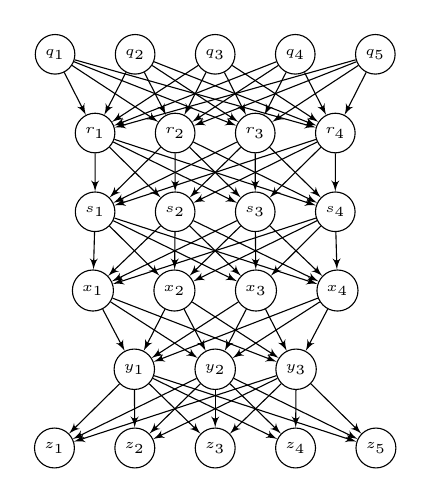
\begin{tikzpicture} \tiny
    %%% Nodes.
    \begin{scope}[]
      \matrix[nodes = {draw, nn}, column sep = 0.5cm] {
        \node (q1) {$q_1$}; &
        \node (q2) {$q_2$}; &
        \node (q3) {$q_3$}; &
        \node (q4) {$q_4$}; &
        \node (q5) {$q_5$}; \\
      };
    \end{scope}
    \begin{scope}[yshift = -1cm]
      \matrix[nodes = {draw, nn}, column sep = 0.5cm] {
        \node (r1) {$r_1$}; &
        \node (r2) {$r_2$}; &
        \node (r3) {$r_3$}; &
        \node (r4) {$r_4$}; \\
      };
    \end{scope}
    \begin{scope}[yshift = -2cm]
      \matrix[nodes = {draw, nn}, column sep = 0.5cm] {
        \node (s1) {$s_1$}; &
        \node (s2) {$s_2$}; &
        \node (s3) {$s_3$}; & \node (s4) {$s_4$}; \\
      };
    \end{scope}
    \begin{scope}[yshift = -3cm]
      \matrix[nodes = {draw, nn}, column sep = 0.5cm] {
        \node (x1) {$x_1$}; &
        \node (x2) {$x_2$}; &
        \node (x3) {$x_3$}; &
        \node (x4) {$x_4$}; \\
      };
    \end{scope}
    \begin{scope}[yshift = -4cm]
      \matrix[nodes = {draw, nn}, column sep = 0.5cm] {
        \node (y1) {$y_1$}; &
        \node (y2) {$y_2$}; &
        \node (y3){$y_3$}; \\
      };
    \end{scope}
    \begin{scope}[yshift = -5cm]
      \matrix[nodes = {draw, nn}, column sep = 0.5cm] {
        \node (z1) {$z_1$}; &
        \node (z2) {$z_2$}; &
        \node (z3) {$z_3$}; &
        \node (z4) {$z_4$}; &
        \node (z5) {$z_5$}; \\
      };
\end{scope}

%%% Edges.
\foreach \q in {1, 2, 3, 4, 5} {
  \foreach \r in {1, 2, 3, 4} {
    \path [line] (q\q) -- (r\r);
  }
}

\foreach \r in {1, 2, 3, 4} {
  \foreach \s in {1, 2, 3, 4} {
    \path [line] (r\r) -- (s\s);
  }
}

\foreach \s in {1, 2, 3, 4} {
  \foreach \x in {1, 2, 3, 4} {
    \path [line] (s\s) -- (x\x);
  }
}

\foreach \x in {1, 2, 3, 4} {
  \foreach \y in {1, 2, 3} {
    \path [line] (x\x) -- (y\y);
  }
}

\foreach \y in {1, 2, 3} {
  \foreach \z in {1, 2, 3, 4, 5} {
    \path [line] (y\y) -- (z\z);
  }
}
  \end{tikzpicture}
  \caption{A Deep Neural Network}
  \label{fig:deep_nn}
\end{figure}

If we let $f_\theta$ denote the neural network parameterized by
$\theta$, we can think of training $f_\theta$ as searching through
$\Theta \subset [0, 1]^n$, the space of all possible
parameterisations, in search of $\theta$ that minimizes some
differentiable measure of loss.

An information theoretic explanation for what deep learning is and how
the training works is given in \cite{ref:tishby-2015} and
\cite{ref:tishby-2017}. Tishby touches on some important topics in
deep learning from an information theory perspective.  One such
assertion of his is the arbitrary nature of the structure of the
graph, i.e.\ there are many equivalent graphs that do the same thing;
the weights at each node do not have meaning. Therefore we are not
searching for some perfect $\theta^* \in \Theta$, as there are many
equivalent $\theta$.

There are many optimization algorithms for searching $\Theta$, most of
which are variations of gradient descent. Gradients are taken with
respect to the loss function $\&L$ and blame is distributed throughout
the graph by the \textit{backpropagation} algorithm. Backpropagation
was introduced in \cite{ref:rumelhart-1986}, and is essentially an
application of the chain rule of calculus to compute the derivatives
of the loss function with respect to each parameter in the graph.

\begin{figure}[H] \centering
  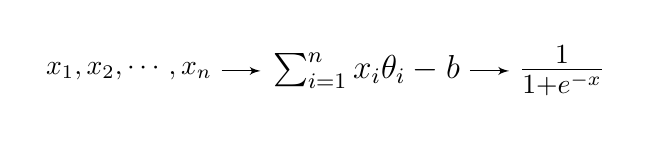
\begin{tikzpicture}
    \begin{scope}[] \matrix[] {
        \node (x1) {$x_1, x_2, \cdots, x_n$}; \\
      };
    \end{scope}
    %%% Summation:
    \begin{scope}[xshift = 3cm]
      \matrix[column sep = -0.2cm] {
        \node (p) {}; &
        \node (sum) {\large $\sum_{i = 1}^n x_i\theta_i - b$}; \\
      };
    \end{scope}
    %%% Activation:
    \begin{scope}[xshift = 5.5cm]
      \matrix[column sep = 1cm] {
        \node (sigma) { \Large ${1 \over 1 + e^{-x}}$}; \\
      };
    \end{scope}
    \path [line] (x1) -- (p); \path [line] (sum) -- (sigma);
  \end{tikzpicture}
  \caption{A Neuron}
  \label{fig:node_of_nn}
\end{figure}

Like a neural network, a linear regression model is a function
parameterized by a set of learnable weights $\theta$. The formula for
linear regression is
\begin{align}
  \label{eq:lin-reg} \hat{y} = \sum_{k=1}^m x_k\theta_k - b.
\end{align} The weight vector $\theta$ of a linear regression model
can be thought of as an expression for how important each entry of
$\mathbf{x}$ is for a specific output $y$. A linear regression model
may also include a bias term $b$, which in the case of a neural
network can be interpreted as the activation threshhold for the
neuron. In a sense, a neural network provides a way to compose many
linear regression models into a much larger
model. \cite{ref:cheng-2018} even go so far as to say that
feed-forward neural networks are equivalent to polynomial regression.

\subsubsection*{Generative Adversarial Networks}

The GAN algorithm comprises two neural networks, the generator $\G$
(and its parameters $\phi$) and the discriminator $\D$ (and its
parameters $\theta$). The generator's parameters $\phi$ are optimized
until $\G$ maps points from a space $\&Z$ to the desired region of
$\&X$ (the sample space). The discriminator's task is more
complicated. $\D$ is optimized until it can correctly classify samples
$\*x$ as either real or fake. $\D$ does this by calculating the
probability that the samples it observes came from true the
distribution $\pt$.

\begin{figure}[H] \centering
  \label{fig:simple_deep_nn} \tiny
  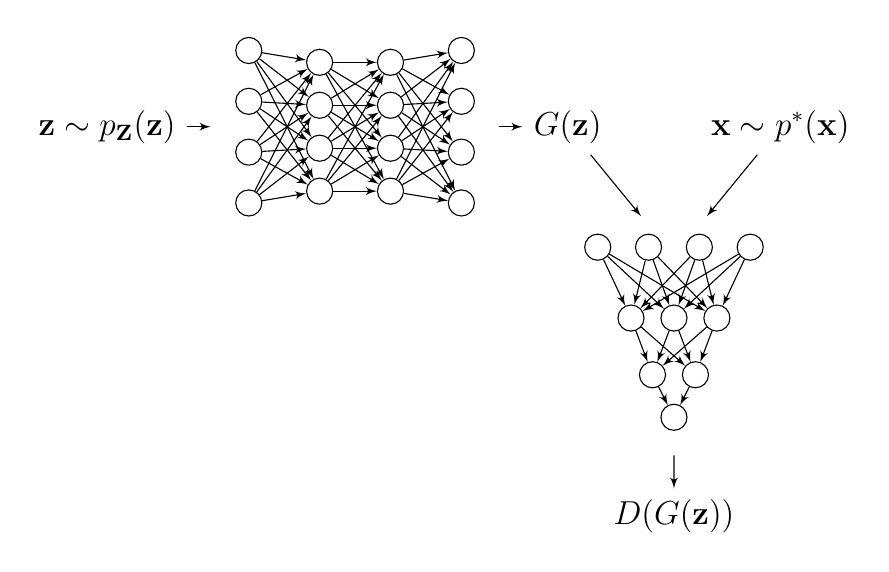
\begin{tikzpicture}[scale = 0.9]
    \begin{scope}
      %%% Noise:
      \begin{scope}[xshift = -5cm] \large
        \node (noise) {$\mathbf{z} \sim p_\mathbf{Z}(\mathbf{z})$};
      \end{scope}
      %%% Transformed Noise
      \begin{scope}[xshift = 1.5cm] \large
        \node (Gz) {$G(\mathbf{z})$};
      \end{scope}
      %%% Transformed Noise
      \begin{scope}[xshift = 4.5cm] \large
        \node (data) {$\mathbf{x} \sim p^*(\mathbf{x})$};
      \end{scope}
      %%% Generator.
      \begin{scope}[xshift = 0.4cm]
        \node (g_output) {};
      \end{scope}
      \begin{scope}[]
        \matrix[nodes = {draw, nn}, row sep = 0.3cm] {
          \node (q1) {}; \\
          \node (q2) {}; \\
          \node (q3) {}; \\
          \node (q4) {}; \\
        };
      \end{scope}
      \begin{scope}[xshift = -1cm]
        \matrix[nodes = {draw, nn}, row sep = 0.2cm] {
          \node (r1) {}; \\
          \node (r2) {}; \\
          \node (r3) {}; \\
          \node (r4) {}; \\
        };
      \end{scope}
      \begin{scope}[xshift = -2cm]
        \matrix[nodes = {draw, nn}, row sep = 0.2cm] {
          \node (s1) {}; \\
          \node (s2) {}; \\
          \node (s3) {}; \\
          \node (s4) {}; \\
        };
      \end{scope}
      \begin{scope}[xshift = -3.4cm]
        \node (g_input) {};
      \end{scope}
      \begin{scope}[xshift = -3cm]
        \matrix[nodes = {draw, nn}, row sep = 0.3cm] {
          \node (x1) {}; \\
          \node (x2) {}; \\
          \node (x3) {}; \\
          \node (x4) {}; \\
        };
      \end{scope}

      %%% Edges.
      \foreach \q in {1, 2, 3, 4} {
        \foreach \r in {1, 2, 3, 4} {
          \path [line] (r\r) -- (q\q);
        }
      }
      \foreach \r in {1, 2, 3, 4} {
        \foreach \s in {1, 2, 3, 4} {
          \path [line] (s\s) -- (r\r);
        }
      }
      \foreach \s in {1, 2, 3, 4} {
        \foreach \x in {1, 2, 3, 4} {
          \path [line] (x\x) -- (s\s);
        }
      }

      %%% Discriminator.
      \begin{scope}[xshift = 3cm, yshift = -1.7cm]
        \begin{scope}[yshift = 0.3cm]
          \matrix[column sep = 0.4cm] {
            \node (d_input_1) {}; &
            \node (d_input_2) {}; \\
          };
        \end{scope}
        \begin{scope}[]
          \matrix[nodes = {draw, nn}, column sep = 0.3cm] {
            \node (q1) {}; &
            \node (q2) {}; &
            \node (q3) {}; &
            \node (q4) {}; \\
          };
        \end{scope}
        \begin{scope}[yshift = -1cm]
          \matrix[nodes = {draw, nn}, column sep = 0.2cm] {
            \node (r1) {}; &
            \node (r2) {}; &
            \node (r3) {}; \\
          };
        \end{scope}
        \begin{scope}[yshift = -1.8cm]
          \matrix[nodes = {draw, nn}, column sep = 0.2cm] {
            \node (s1) {}; & \node (s2) {}; \\
          };
        \end{scope}
        \begin{scope}[yshift = -2.4cm]
          \matrix[nodes = {draw, nn}, column sep = 0.2cm] {
            \node (x1) {}; \\
          };
        \end{scope}

        \begin{scope}[yshift = -2.8cm]
          \node (d_output) {};
        \end{scope}

        %%% Edges.
        \foreach \q in {1, 2, 3, 4} {
          \foreach \r in {1, 2, 3} {
            \path [line] (q\q) -- (r\r);
          }
        }
        \foreach \r in {1, 2, 3} {
          \foreach \s in {1, 2} {
            \path [line] (r\r) -- (s\s);
          }
        }
        \foreach \s in {1, 2} {
          \foreach \x in {1} {
            \path [line] (s\s) -- (x\x);
          }
        }
      \end{scope}

      \begin{scope}[xshift = 3cm, yshift = -5.5cm]
        \large \node (p) {$D(G(\*z))$};
      \end{scope}

      \path [line] (noise) -- (g_input);
      \path [line] (g_output) -- (Gz);
      \path [line] (Gz) -- (d_input_1);
      \path [line] (data) -- (d_input_2);
      \path [line] (d_output) -- (p);

    \end{scope}
  \end{tikzpicture}
  \caption{The Architecture of the GAN Algorithm}
\end{figure}

The generator of the GAN algorithm trains a \textit{generative model},
which we define as any mathematical or statistical model that mimics
the process of creating the observed data \cite{ref:bishop}. Starting
with randomly initialized parameters, which means we randomly choose a
$\theta \in \Theta$, we optimize the model until it maps random input
into the desired output with frequencies similar enough to the desired
probability distribution. In other words we take a random vector $\*Z
= \left\{Z_1, Z_2, \dots, Z_n\right\}$, where each $Z_i \sim
\mathcal{N}(0, 1)$ is a normally distributed random variable with mean
0 and variance 1 (we could also use a random input following a
different distribution).
\begin{align}
  \label{eq:gen-model} f_\theta(\*Z): \*Z \mapsto \&X
\end{align} We then pass $\*Z$ through a parametric function which
does the transformation, and we obtain a sample from the target space
$\&X$.

The earliest reference to two-player games that result in the
production of a generative model can be found in \cite{ref:doyle}, a
short article containing the following game. \textit{``We are told the
constraints, we pick a distribution, God gets to pick the `real'
distribution, satisfying the constraints of course. Some disinterested
party picks an outcome according to the `real' distribution that God
has just picked, and we have to pay according to how surprised we are
to see that outcome.''} This is not quite the GAN algorithm, but it
has a similar moral, that is we seek a probability distriution and we
learn what qualities define it through feedback. If we iterate the
above procedure and formalize a way of learning from our surprise, we
arrive at something resembling the GAN algorithm.

As for the history of adversarial games (where the players are trying
to undermine each other), J\"{u}rgen Schmidhuber wrote more than one
paper, the first of which appeared in 1992, on what he called
``predictability minimization'', which is very similar to the GAN
algorithm (see \cite{ref:schmidhuber-1992} and
\cite{ref:schmidhuber-2018}). The idea behind \textit{predictability
minimization} was for one player to try to predict outcomes in some
event space and the adversary tries to minimize the ability of that
player to make those predictions.

A blog post from 2010 essentially describes the GAN algorithm, see
\cite{ref:niemitalo-2010}. In 2012, a paper on adversarial support
vector machines was written by \cite{ref:zhou-2012}. Finally, in 2014
an algorithm for training models to simulate the behaviour of animals
based on two populations, replicas and classifiers, was written by
\cite{ref:li-2014}.

In 2014, while a student of Yoshua Bengio at the Universit\'{e} de
Montr\'{e}al, Ian Goodfellow and colleagues published
\textit{Generative Adversarial Nets}.  This paper has since inspired
many publications and has triggered a surge in the interest in
generative models.

%%% Local Variables: %%% mode: latex %%% TeX-master: "../thesis.tex"
%%% TeX-master: "../thesis"
%%% End:

% Game Theory Chapter
\section{Game Theory}%
\label{sec:game-theory}
\vspace{0.5cm}
\begin{figure}[h!]%
  \label{fig:paradise-2}
  \centering
  \fcolorbox{black}{white}{
    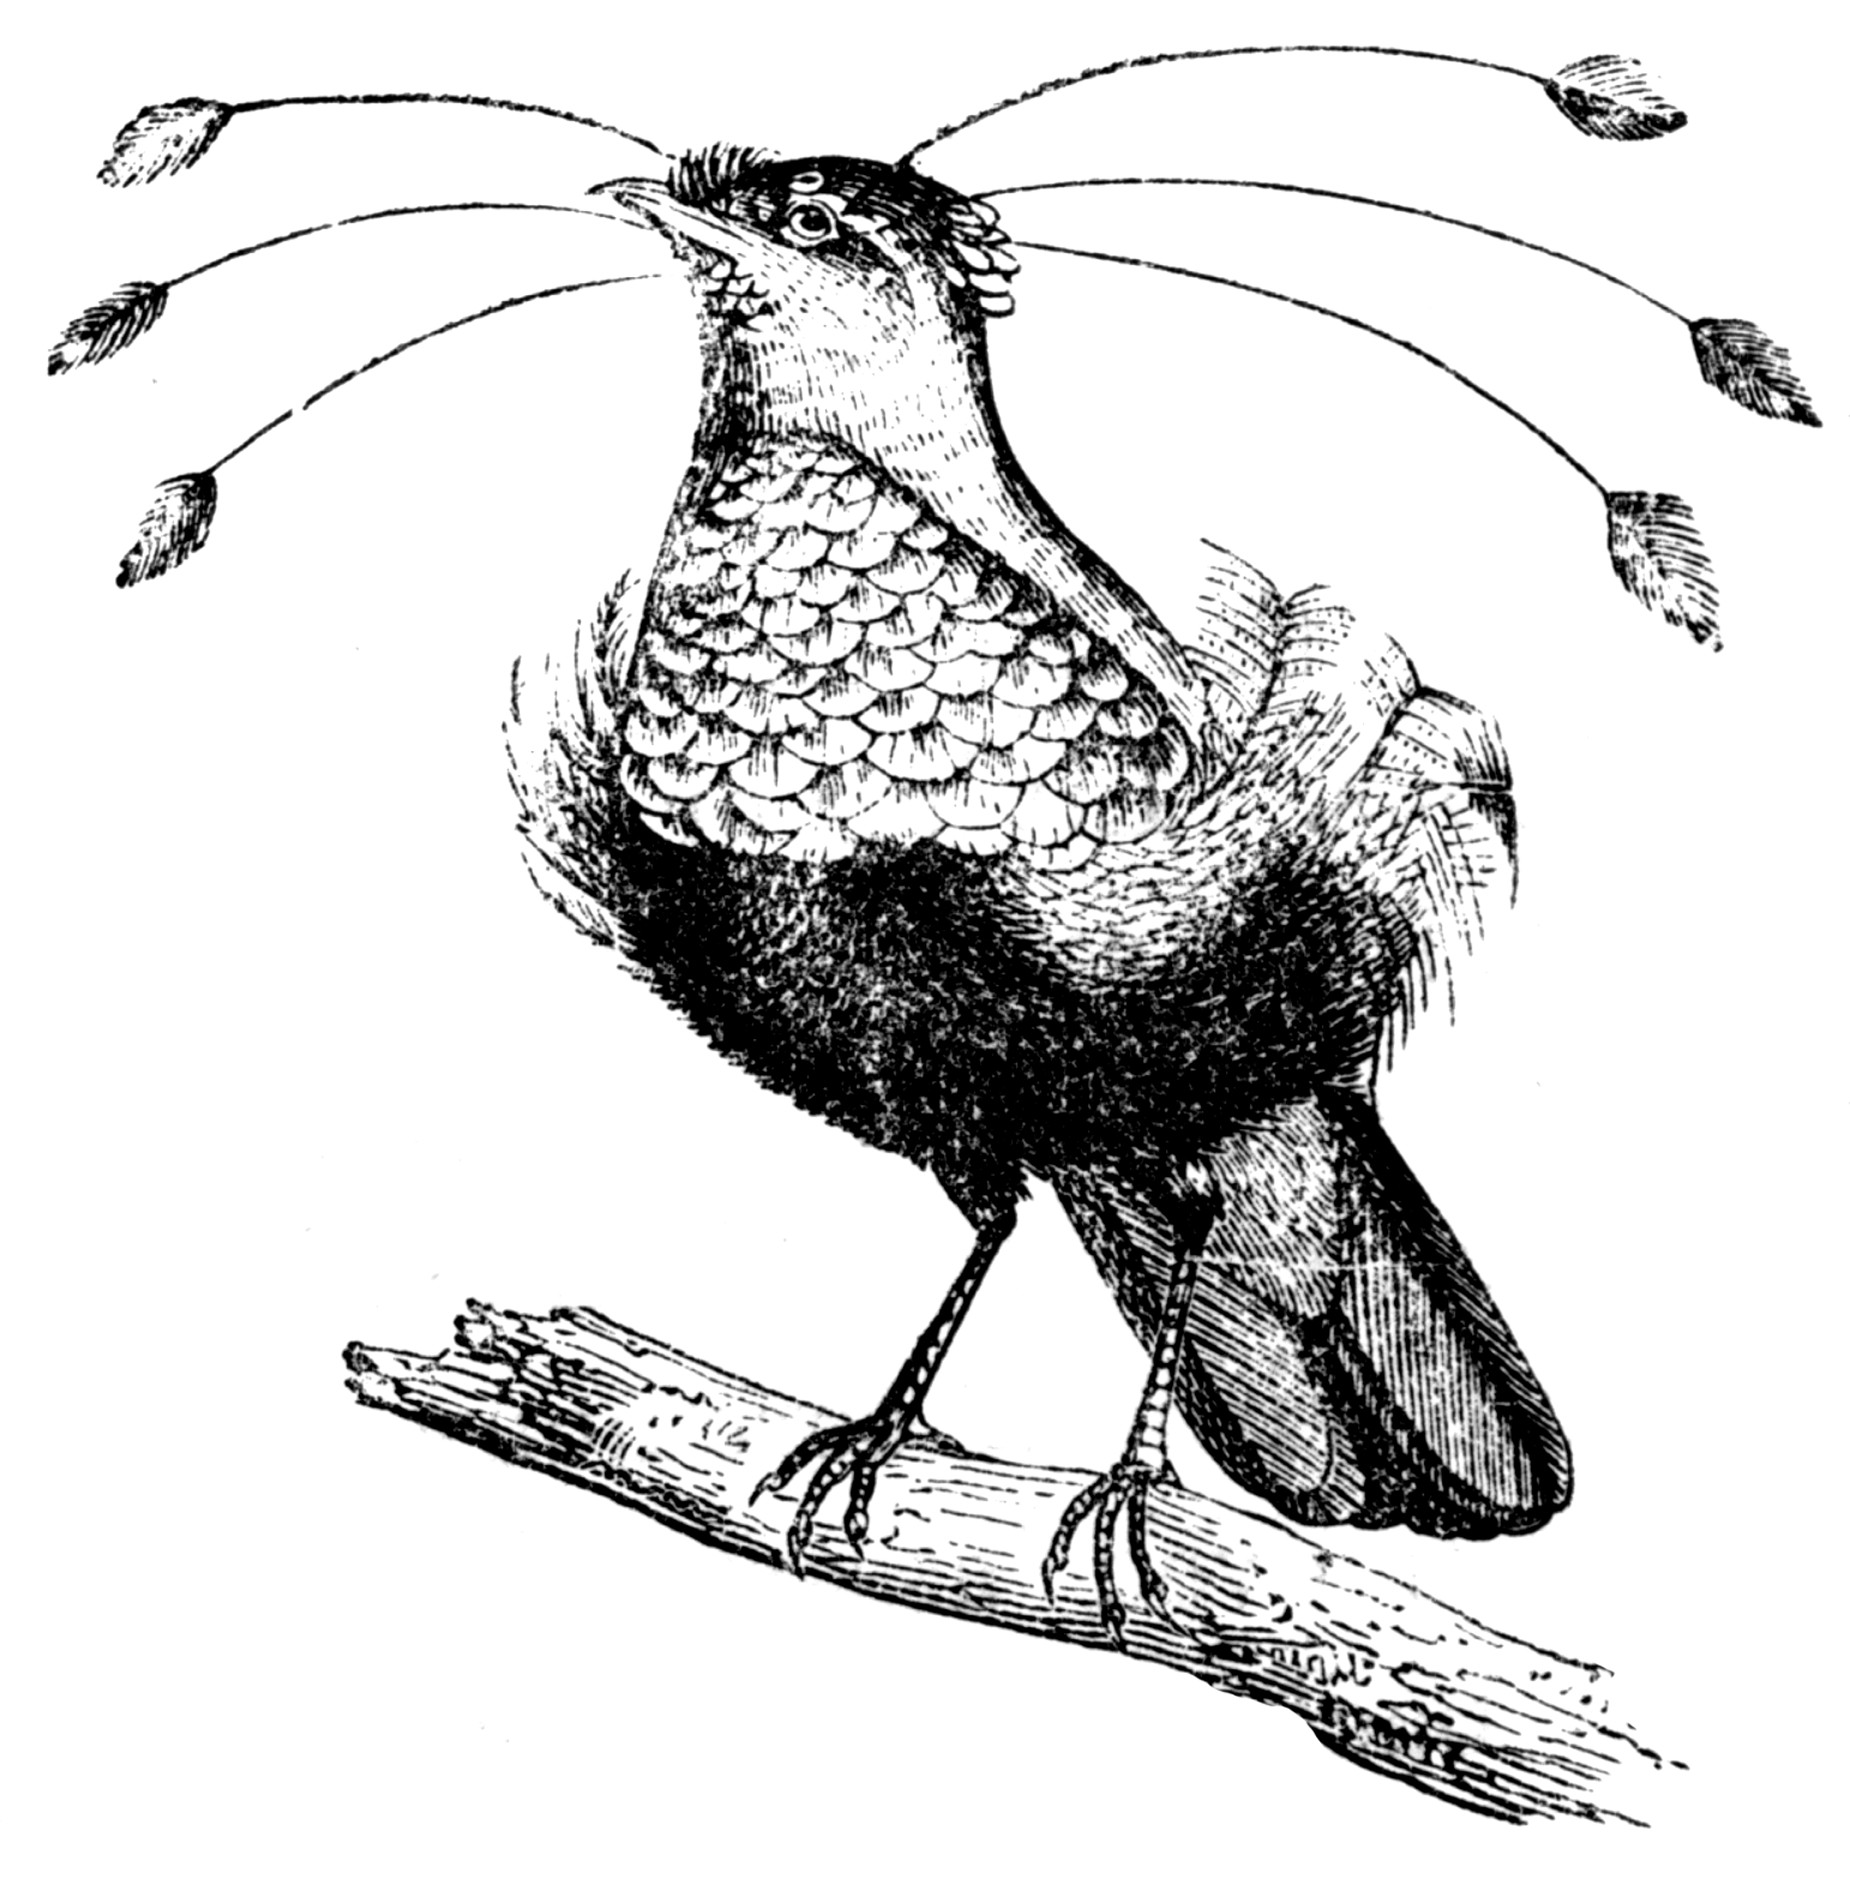
\includegraphics[width=0.3\textwidth]{paradise}
  }
  \caption{Louis Figuier, ``Reptiles and Birds'', 1869. This artwork symbolizes the adversarial relationship in game theory, where different entities compete for dominance, much like the generator and discriminator in GANs.}
\end{figure}
\vspace{0.5cm}

The Generative Adversarial Network (GAN) framework is fundamentally rooted in game theory, which studies strategic interactions between rational decision-makers using mathematical models~\cite{ref:myerson}. In this section, we examine GANs through the lens of two-player games, where the discriminator ($D$) and generator ($G$) engage in an adversarial competition. We denote their value functions as $V_D$ and $V_G$, respectively.

\subsection{Game-Theoretic Foundations}

\begin{definition}%
  \label{def:value-function}
  A \textnormal{\sffamily value function} $V_i$ quantifies the reward (or loss if negative) for player $i$ in a game, expressed as a function of the player's actions.
\end{definition}

\begin{remark}
  In many machine learning contexts, the loss function represents the difference between target values $y$ and estimates $\hat{y}$. In GANs, however, the value function is more complex, serving as a measure of uncertainty in the adversarial game.
\end{remark}

The original GAN formulation~\cite{ref:goodfellow-original} introduces two value functions. The first frames GANs as a zero-sum game, while the second provides a more practical training objective~\cite{ref:gidel-variational-2018}.

\begin{definition}%
  \label{def:zero-sum-game}
  A \textnormal{\sffamily zero-sum game} is one where one player's gain exactly equals the other player's loss. Formally, $V_D + V_G = 0$.
\end{definition}

\begin{remark}
  For this section, we focus on the zero-sum formulation, where the GAN algorithm represents a strategic competition between the generator and discriminator (see Definitions~\ref{def:generator} and~\ref{def:discriminator}).
\end{remark}

\subsection{Minimax Strategy and Equilibrium}

In zero-sum games, players seek optimal strategies to maximize their minimum possible reward. The minimax decision rule provides a framework for this optimization.

\begin{definition}
  \label{def:minimax}
  In a two-player game with players $D$ and $G$, the \textnormal{\sffamily minimax decision rule} for $D$ maximizes $D$'s expected reward after $G$ has minimized $D$'s maximum attainable reward. The \textnormal{\sffamily minimax value} $\overline{V_D}$ is:
  \begin{align}
    \overline{V_D} = \min_{G} \max_{D} V_D(D, G).
  \end{align}
\end{definition}

The minimax strategy ensures the best possible outcome against an optimal opponent. If $G$ moves first to minimize $D$'s reward, $D$'s minimax rule maximizes the reduced reward.

\subsection{Nash Equilibrium and Strategic Stability}

The GAN algorithm seeks a Nash equilibrium in the parameter space of the discriminator and generator~\cite{ref:goodfellow-2016,ref:goodfellow-2017}.

\begin{definition}
  A \textnormal{\sffamily Nash equilibrium} in an $n$-player game is a strategy profile $s^* = (s_1, s_2, \dots, s_n)$ where no player can benefit by unilaterally changing their strategy. Formally, for all players $i$ and alternative strategies $s_{-i}$:
  \begin{align}
    f_i(s^*) \geq f_i(s_1, s_2, \dots, s_{-i}, \dots, s_n)
  \end{align}
  where $f_i(s)$ is the payoff to player $i$ under strategy profile $s$.
\end{definition}

\begin{remark}
  In a Nash equilibrium, each player's strategy is optimal given the others' strategies. For zero-sum games, the minimax solution corresponds to a Nash equilibrium. Note that Nash equilibria are not necessarily globally optimal, and multiple equilibria may exist.
\end{remark}

\subsubsection{Prisoner's Dilemma: A Case Study}
\label{sec:prisoners-dilemma}

The Prisoner's Dilemma illustrates key concepts of Nash equilibrium and strategic interaction. Originally formulated by Flood and Dresher in the 1950s and later reformulated by Tucker~\cite{ref:poundstone}, it demonstrates how individual rationality can lead to suboptimal collective outcomes.

In this game, two players ($D$ and $G$) are held in separate custody with no communication. Each faces the following choices:
\begin{enumerate}
  \item If one defects (accuses the other) while the other denies, the defector receives 1 year (reward for cooperation) while the other receives 5 years.
  \item If both deny, each receives 2 years (sufficient evidence exists for the lesser crime).
  \item If both defect, each receives 3 years.
\end{enumerate}

\begin{figure}[h]
  \centering%
  \bgroup%
  \def\arraystretch{1.4}
  \begin{tabular}[c]{|c|c|c|}
    \hline
    \diagbox{$D$}{$G$} & Deny  & Defect \\
    \hline
                  Deny & (2, 2) & (5, 1) \\
    \hline
                Defect & (1, 5) & (3, 3) \\
    \hline
  \end{tabular}
  \egroup
  \caption{Prisoner's Dilemma payoff matrix (years in prison for $D$, $G$). The global optimum (Deny, Deny) is unstable, while (Defect, Defect) is the Nash equilibrium.}%
  \label{fig:prisoners-matrix}
\end{figure}

Analyzing all possible states:
\begin{enumerate}
  \item \textbf{(Deny, Defect)}: If $D$ switches to defect while $G$ defects, $D$ improves from 5 to 3 years. This is not a Nash equilibrium (and symmetrically for (Defect, Deny)).
  
  \item \textbf{(Deny, Deny)}: If $D$ switches to defect while $G$ denies, $D$ improves from 2 to 1 year. This is not a Nash equilibrium.
  
  \item \textbf{(Defect, Defect)}: Neither player can improve by unilaterally changing strategy. If $D$ switches to deny while $G$ defects, $D$ worsens from 3 to 5 years. This is the Nash equilibrium.
\end{enumerate}

This example shows that the globally optimal outcome (Deny, Deny) is unstable, while the Nash equilibrium (Defect, Defect) is stable but suboptimal. This has important implications for GANs, as we'll see later.

\subsection{Derivation of the GAN Value Function}%
\label{sec:derivation}

We now derive the GAN value function from game-theoretic principles. Let $(\mathcal{X}, p_{data})$ be a probability space where $\mathcal{X}$ is a finite space (e.g., the space of all $H \times W$ 8-bit RGB images, $\mathcal{X} = [0, 255]^{3 \times H \times W}$) and $p_{data}$ assigns mass to regions corresponding to meaningful images.

The GAN algorithm trains a generator $G_\phi$ (parameterized by $\phi \in \Phi \subset \mathbb{R}^n$) to map random samples $z$ from a prior space $(\mathcal{Z}, p_z)$ to $\mathcal{X}$ such that $G_\phi(z)$ lies in regions where $p_{data}$ assigns significant mass. Typically, $\mathcal{Z} \neq \mathcal{X}$ and $|\mathcal{Z}| < |\mathcal{X}|$~\cite{ref:arjovsky-2017}.

\begin{figure}[H]
  \centering
  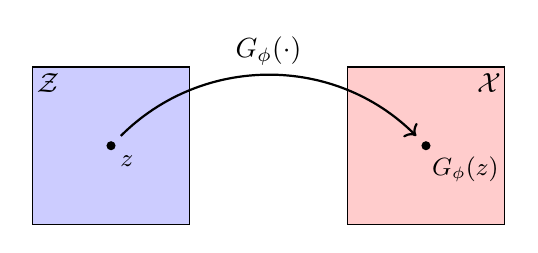
\begin{tikzpicture}
    \node (G) at (3, 2.2) {$G_\phi(\cdot)$};
    \draw[fill=blue!20] (0, 0) rectangle +(2, 2);
    \node at (0.2, 1.8) {$\mathcal{Z}$};
    \filldraw (1, 1) circle (0.05cm);
    \node (Z) at (1, 1) {};
    \node (ZZ) at (1.2, 0.8) {\small $z$};
    \draw[fill=red!20] (4, 0) rectangle +(2, 2);
    \filldraw (5, 1) circle (0.05cm);
    \node (O) at (5, 1) {};
    \node (OO) at (5.5, 0.7) {\small $G_\phi(z)$};
    \node at (5.8, 1.8) {$\mathcal{X}$}; 
    \draw[->,thick] (Z) to [out=45,in=135] (O);
  \end{tikzpicture}
  \caption{The generator $G_\phi$ transforms noise $z \sim p_z$ into synthetic samples $G_\phi(z) \in \mathcal{X}$. The goal is for these samples to lie in high-probability regions under $p_{data}$.}%
  \label{fig:g-maps}
\end{figure}

Initially, $G_\phi$ maps $z$ to $\mathcal{X}$ randomly. Through adversarial training, both $D_\theta$ and $G_\phi$ learn $p_{data}$ from different perspectives: $D_\theta$ learns to distinguish real from generated samples, while $G_\phi$ learns to generate samples that fool $D_\theta$.

The value function $V$ captures this adversarial dynamic:
\begin{align}
  \label{eq:the-original-objective-function}
  V(D_\theta, G_\phi) = \mathbb{E}_{x \sim p_{data}}[\log D_\theta(x)] + \mathbb{E}_{z \sim p_z}[\log(1 - D_\theta(G_\phi(z)))].
\end{align}

This value function resembles the noise-contrastive estimator~\cite{ref:gutmann-2010}. In the game between $G_\phi$ and $D_\theta$, each seeks to maximize their minimum reward by playing their minimax decision rule.

\subsubsection{Discriminator's Objective}%
\label{sec:derivation-d}

From $D_\theta$'s perspective, we want $D_\theta(x)$ to approximate $p_{data}(x)$. We find $\theta \in \Theta$ that maximizes the likelihood:
\begin{align}
  \label{eq:d-1}
  L_D^{(1)}(\theta) = \prod_{i=1}^n D_\theta(x_i), \quad x_i \sim p_{data}.
\end{align}

For numerical optimization, we maximize the log-likelihood:
\begin{align}
  \label{eq:d-l1}
  \ell_D^{(1)}(\theta) = \sum_{i=1}^n \log D_\theta(x_i).
\end{align}

Simultaneously, $D_\theta$ must assign low probability to generated samples $G_\phi(z) = \tilde{x}$. For fixed $G_\phi$, $\theta$ should minimize:
\begin{align}
  ^*L_D^{(2)}(\theta) = \prod_{i=1}^n D_\theta(G_\phi(z_i)), \quad z_i \sim p_z.
\end{align}

Equivalently, we minimize the log-likelihood:
\begin{align}
  \label{eq:d-l2} ^*\ell_D^{(2)}(\theta) = \sum_{i=1}^n \log D_\theta(G_\phi(z_i)).
\end{align}

To combine both objectives, we maximize the complement:
\begin{align}
  \ell_D^{(2)}(\theta) = \sum_{i=1}^n \log(1 - D_\theta(G_\phi(z_i))),
\end{align}

since minimizing $D_\theta(G_\phi(z))$ is equivalent to maximizing $1 - D_\theta(G_\phi(z))$. Combining both objectives, $D_\theta$ maximizes:
\begin{align}
  \sum_{i=1}^n \left( \log D_\theta(x_i) + \log(1 - D_\theta(G_\phi(z_i))) \right).
\end{align}

By the law of large numbers, this sample average converges to:
\begin{align}
  \label{eq:objective-for-d}
  \mathbb{E}_{x \sim p_{data}}[\log D_\theta(x)] + \mathbb{E}_{z \sim p_z}[\log(1 - D_\theta(G_\phi(z)))]
\end{align}
for sufficiently large $n$.

\subsubsection{Generator's Objective}%
\label{sec:derivation-g}

From $G_\phi$'s perspective, we seek $\phi$ that maximizes the likelihood (as judged by a fixed $D_\theta$) that generated samples come from $p_{data}$. We maximize:
\begin{align}
  ^*\ell_G(\phi) = \sum_{i=1}^n \log D_\theta(G_\phi(z_i)), \quad z_i \sim p_z.
\end{align}

Equivalently, we minimize:
\begin{align}
  \ell_G(\phi) = \sum_{i=1}^n \log(1 - D_\theta(G_\phi(z_i))),
\end{align}
which corresponds to minimizing $\mathbb{E}_{z \sim p_z}[\log(1 - D_\theta(G_\phi(z)))]$.

\subsubsection{Minimax Formulation}

The training objectives lead to the minimax formulation:
\begin{align}
  \overline{V_D} & = \min_{\phi}\max_{\theta} V_D(\theta, \phi) \\
                  & = \min_{\phi}\max_{\theta} \left( \mathbb{E}_{x \sim p_{data}}[\log D_\theta(x)] + \mathbb{E}_{z \sim p_z}[\log(1 - D_\theta(G_\phi(z)))] \right)
\end{align}

We solve this by finding the minimax decision rule and value for $D_\theta$ (Theorem~\ref{theorem:minimax}), which corresponds to the Nash equilibrium. However, finding this equilibrium is often challenging in practice.

\subsection{Challenges in Finding Nash Equilibrium}%
\label{sec:difficulty}

Finding Nash equilibria can be difficult, as demonstrated by the following example inspired by~\cite{ref:weng-2017}:

\begin{example}[Oscillatory Dynamics]
  Let $V(x, y) = xy$ be a value function with the game:
  \begin{align}
    \min_x \max_y V(x, y) = xy.
  \end{align}
  
  The gradients are $\frac{\partial V}{\partial x} = y$ and $\frac{\partial V}{\partial y} = x$, leading to updates:
  \begin{align}
    x^{(t+1)} & \gets x^{(t)} - \eta \cdot y, \\
    y^{(t+1)} & \gets y^{(t)} + \eta \cdot x,
  \end{align}
  where $\eta > 0$ is the learning rate.
  
  The Nash equilibrium is $s^* = (s_G^*, s_D^*) = (0, 0, \dots)$, where $V(s_G^*, s_D) = 0$ for all $s_D$, and $V(s_G, s_D^*) = 0$ for all $s_G$.
  
  \begin{figure}[H]
    \centering
    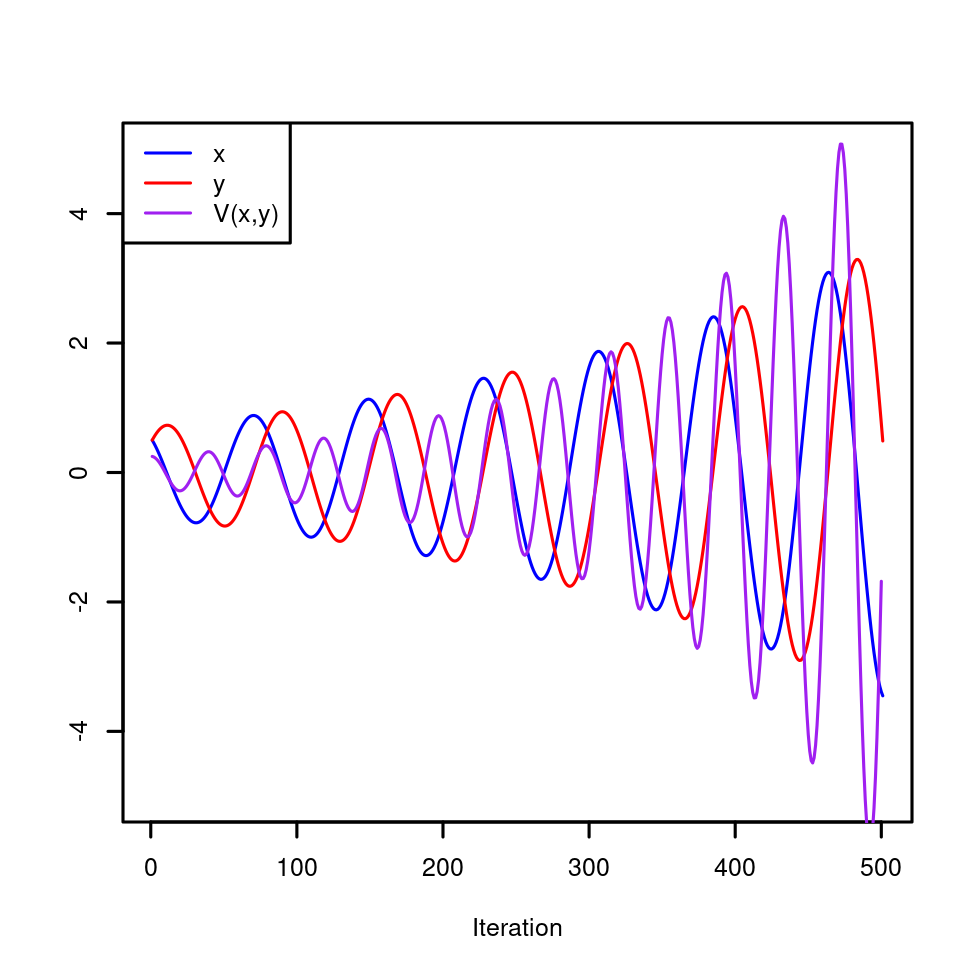
\includegraphics[width=0.6\textwidth]{plot1}
    \caption{Oscillatory behavior around the Nash equilibrium. This pattern is commonly observed in GAN training, where generator and discriminator parameters oscillate rather than converging to a stable equilibrium.}%
    \label{fig:alternating}
  \end{figure}
\end{example}

This oscillatory behavior is frequently observed in GAN training, where alternating gradient updates can cause the system to oscillate around equilibrium rather than converge to it.

\subsection{Alternative Value Functions}%
\label{sec:two-value}

The original value function (Equation~\ref{eq:the-original-objective-function}) often leads to vanishing gradients, especially early in training when $D_\theta$ easily distinguishes real from generated samples. To address this,~\cite{ref:goodfellow-original} introduced an alternative formulation:

\begin{align}
  \label{eq:second-value-function} 
  \max_{\theta} \left( \mathbb{E}_{x \sim p_{data}}[\log D_\theta(x)] + \mathbb{E}_{z \sim p_z}[\log(1 - D_\theta(G_\phi(z)))] \right) \\
  \max_{\phi} \mathbb{E}_{z \sim p_z}[\log D_\theta(G_\phi(z))]
\end{align}

These decoupled objectives share the same fixed points as the original formulation but provide stronger gradients for the generator, improving learning dynamics. With this formulation, GANs are no longer strictly zero-sum games.

\subsection{GAN Algorithm}

The complete GAN algorithm is presented below:

\begin{figure}[H] \centering
  \begin{minipage}{0.95\linewidth}
    \begin{algorithm}[H]
      \SetAlgoLined
      \KwIn{Learning rate $\eta > 0$, Number of iterations $T > 0$}
      \KwOut{Trained discriminator $D_\theta$ and generator $G_\phi$}
      Initialize discriminator parameters $\theta$ and generator parameters $\phi$ randomly\;
      \For{$t = 1$ \KwTo $T$}{
        \textbf{// Update discriminator}\;
        Sample batch $\{x_1, \dots, x_m\}$ from real data distribution $p_{data}$\;
        Sample batch $\{z_1, \dots, z_m\}$ from prior noise distribution $p_z$\;
        Compute discriminator loss:
        \[
        L_D = -\frac{1}{m} \sum_{i=1}^m \left[ \log D_\theta(x_i) + \log(1 - D_\theta(G_\phi(z_i))) \right]
        \]
        Update discriminator parameters: $\theta \gets \theta - \eta \cdot \nabla_\theta L_D$\;
        
        \textbf{// Update generator}\;
        Sample batch $\{z_1, \dots, z_m\}$ from prior noise distribution $p_z$\;
        Compute generator loss:
        \[
        L_G = -\frac{1}{m} \sum_{i=1}^m \log D_\theta(G_\phi(z_i))
        \]
        Update generator parameters: $\phi \gets \phi - \eta \cdot \nabla_\phi L_G$\;
      }
      \caption{Generative Adversarial Networks Algorithm}
      \label{algo:main-algo}
    \end{algorithm}
  \end{minipage}
\end{figure}

Note that in the original paper, the discriminator is updated $k$ times per generator update (typically $k=1$). We've omitted this inner loop for clarity, but it can be important for stability in practice.

\subsection{Strategic Interpretation and Discussion}

The minimax strategy for $D_\theta$ has an important interpretation: if $D_\theta$ assumes $G_\phi$ has done its worst (i.e., generated perfect samples), then $D_\theta$ should assign probability $1/2$ to all inputs. This is the maximum entropy distribution over the two states (real or synthetic), representing maximum uncertainty.

When $D_\theta(x) = 1/2$ for all $x$, the generator receives no useful gradient signal and cannot improve. This represents a strategic equilibrium where neither player can benefit by unilaterally changing their strategy. In the next section, we'll show that $D_\theta(x) = 1/2$ is indeed the optimal strategy for $D_\theta$ at equilibrium.

This game-theoretic perspective reveals fundamental challenges in GAN training:
\begin{itemize}
  \item The minimax formulation can lead to oscillatory dynamics rather than stable convergence
  \item The zero-sum assumption may not hold in practice, as both networks ultimately benefit from reaching a good equilibrium
  \item Alternative value functions can improve training stability by providing better gradient signals
\end{itemize}

Understanding these strategic dynamics is crucial for developing improved GAN variants and training procedures, as we'll explore in subsequent sections.

%%% Local Variables:
%%% mode: latex
%%% TeX-master: "../thesis.tex"
%%% End:

% Information Theory Chapter
\section{Information Theory}%
\label{sec:information-theory}

\vspace{1cm}

\begin{figure}[h!]%
  \label{fig:info}
  \centering
  \fcolorbox{black}{white}{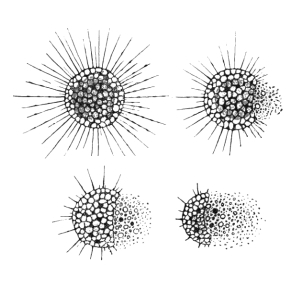
\includegraphics[width=0.3\textwidth]{entropy}}
  \caption{\href{https://www.consciousentities.com/2017/02/consciousness-entropy/}{Conscious
      Entities, Peter Hankins}}
\end{figure}

\vspace{1cm}

\noindent Information theory was born in 1948 with the publication of \textit{A
  Mathematical Theory of Communication} by Claude Shannon
(1916~\textendash~2001). Shannon was inspired in part by earlier work by
Boltzmann and Gibbs in thermodynamics and by Hartley and Nyquist at Bell,
see~\cite{ref:losee-1997}. Most of the theory and applications of information
theory (compression, coding schemes, data transfer over noisy channels) are
outside the scope of this thesis, but there are certain information theoretic
quantities used regularly in machine learning, so it is useful to discuss them
now.

\begin{remark}
  The information we talk about is restricted to the information about the
  probability distribution over the elementary outcomes, not information about
  the content of the outcomes. The significance of probability is that it tells
  us how certain we can be when making inference. The most important information
  in this regard is found in the probability distribution over the possible
  outcomes.
\end{remark}

Information theory is quite useful for deep learning. If we think of neural nets
as noisy channels, the need for this theory becomes even more obvious.
In~\cite{ref:mackay-2003}, David Mackay said ``brains are the ultimate
compression and communication systems. And the state-of-the-art algorithms for
both data compression and error-correcting codes use the same tools as machine
learning''. Furthermore, ``we might anticipate that the best data compression
algorithms will result from the development of artificial intelligence
methods''.

The most fundamental quantity in information theory is entropy. Before we state
the formal definition of entropy, we will motivate it as a measure of
uncertainty by walking through its derivation. We will define a function $\eta$
as a measure of uncertainty and we will derive entropy as a function based on
the requirements it must satisfy using $\eta$ as a starting point.

\begin{definition}
  Let $(\&X, p)$ be a discrete probability space. We define
  \textnormal{\sffamily uncertainty} to be a real-valued function
  $\eta(\cdot): \&X \mapsto \R^+$ which depends only on the
  probabilities of the elementary outcomes and satisfies the
  following:
  \begin{enumerate}[(i)]
  \item If an outcome $x$ is guaranteed to occur, then there is no
    uncertainty about it and $\eta(x) = 0$;
  \item For any two outcomes $x$, $x^\prime$, we have $p(x) < p(x^\prime) \iff
    \eta(x) > \eta(x^\prime)$;
  \item For any two independent outcomes, $x$, $x^\prime$, the
    uncertainty of their joint occurrence, is the sum of their
    uncertainties, i.e.
    $\eta(x \cdot x^\prime) = \eta(x) + \eta(x^\prime)$.
  \end{enumerate}
\end{definition}
\begin{remark}
  This definition is a modification of one given
  by~\cite{ref:martin-2011}.
\end{remark}

It should not be a surprise that it is new information we are interested in,
since that is what reduces uncertainty. Common outcomes provide less information
than rare outcomes, which means $\eta$ should be inversely proportional to the
probability of the outcome.
\begin{align}
  \label{eq:eta-1}
  \eta(x) \propto {1 \over p(x)}
\end{align}
Since $\eta$ must satisfy $\eta(x \cdot x^\prime) = \eta(x) + \eta(x^\prime)$,
we must define $\eta$ in terms of the logarithm. This is because the probability
of two independent outcomes is the product of their probabilities whereas we
want information to be additive.  Thus,
\begin{align}
  \label{eq:eta-3}
  \eta(x) \approx \log{1 \over p(x)}.
\end{align}
For probability distributions, we need a measure of uncertainty that says, on
average, how much uncertainty is contained in $(\&X, p)$. We need to weight the
calculation by the probability of observing each outcome. This means what we are
really seeking is a measure on the probability distribution over $\&X$. We
adjust the notation, using the capital eta, which resembles the Latin H. Thus,
\begin{align}
  \label{eq:eta-almost}
  \&H(p) = \sum_{x \in \&X} p(x) \log{1 \over p(x)}.
\end{align}
This is what we will call entropy, a measure on the average amount of surprise
associated to outcomes from $(\&X, p)$. Entropy is maximized when we cannot say
with any confidence if an outcome will occur. This upper bound occurs when the
probabilities over the set of possible outcomes are uniformly distributed.
\begin{align}
  \label{eq:eta-2}
  \&H(p) \leq \log{|\&X|}
\end{align}
We can also think of entropy as how much information, measured in binary
information units (bits), is required to describe outcomes drawn from $(\&X,
p)$. The way to understand this last part is the logarithm tells us how many
bits we need to describe this uncertainty, since
\begin{align}
  \label{eq:understand-log}
  \log_2{1 \over p(x)} = n \iff 2^n = {1 \over p(x)}.
\end{align}
However, any logarithm can be used. Base $e$ and base 10 are also commonly used.
\begin{definition}
  Let $(\&X, p)$ be any discrete probability space. The \textnormal{\sffamily
    entropy} of a probability distribution $p$ with mass function $p$, denoted
  by $\&H(p)$, is the average amount of uncertainty found in elementary outcomes
  from $(\&X, p)$. We write
  \begin{align}
    \label{eq:entropy}
    \&H(p) = - \mathbb{E}_{x \sim p} \left[ \log{p(x)} \right].
  \end{align}
  The entropy of a probability distribution tells us how much
  variation we should expect to see in samples drawn from $(\&X,
  p)$. The probability distribution with maximum entropy is the
  uniform distribution since all outcomes are equally surprising.
\end{definition}

Figure~\ref{fig:entropy-coin-toss} depicts the entropy of a
probability distribution over two states as a function of the symmetry
of the distribution.  As the probability of heads $p(H)$ approaches 0
or 1, we see the uncertainty vanishes, and uncertainty is maximized
when probability is equally distributed over heads and tails.

\begin{figure}[H]
  \centering
  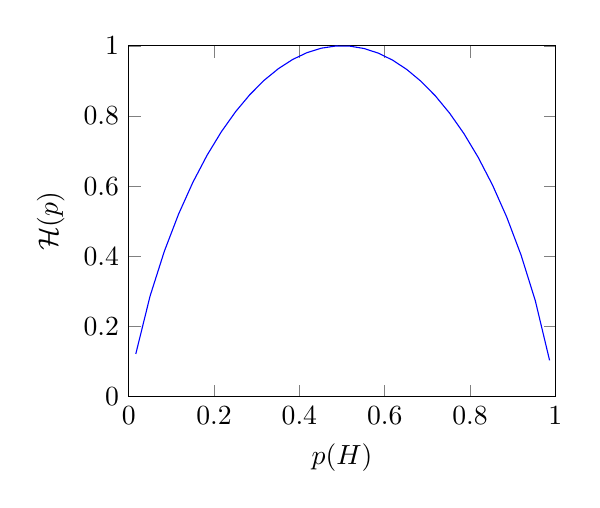
\begin{tikzpicture}
    \begin{axis}[
      ymin = 0,
      ymax = 1,
      xmin = 0,
      xmax = 1,
      xlabel = $p(H)$,
      ylabel = $\&H(p)$,
      enlargelimits = false]
      \addplot [samples = 300, blue] {-x*log2(x)-(1-x)*log2(1-x)};
    \end{axis}
  \end{tikzpicture}
  \caption{Entropy of a coin toss as a function of the symmetry of $p(H)$.}%
  \label{fig:entropy-coin-toss}
\end{figure}

\begin{example}
  The entropy of the probability distribution corresponding to a fair coin toss
  is 1 bit, and the entropy of $m$ tosses is $m$ bits. If there are two states
  of equal probability, then we need 1 bit and if we have 3 states of equal
  probability, we need 1.584963 bits.
\end{example}

\subsubsection*{Entropy-based Quantities}

We include a definition of a metric below in order to make clear the distinction
between it and a divergence, which will be defined afterwards.

\begin{definition}
  A \textnormal{\sffamily metric} on a set $\&X$ is a function $d(\cdot, \cdot): \&X \times
  \&X \mapsto \R^+$ such that, $\forall x, y, z \in \&X$:
  \begin{enumerate}
  \item $d(x, y) \geq 0$, and $d(x, y) = 0 \iff x = y$
  \item $d(x, y) = d(y, x)$
  \item $d(x, z) \leq d(x, y) + d(y, z)$
  \end{enumerate}
\end{definition}

\begin{remark}
  A divergence is a weaker notion than that of distance. A divergence
  need not be symmetric nor satisfy the triangle inequality.
\end{remark}

\begin{definition}
  Let $\&P$ be any space of probability distributions over any finite
  set $\&X$ such that all $P \in \&P$ have the same support. A
  \textnormal{\sffamily divergence} on $\&P$ is a function,
  $\&D\left( \cdot \mid\mid \cdot \right): \&P \times \&P \mapsto
  \R^+$, such that $\forall p, q \in \&P$ the following conditions are
  satisfied
  \begin{enumerate}[(i)]
  \item $\&D(p||q) \geq 0$
  \item $\&D(p||q) = 0 \iff p = q$.
  \end{enumerate}
\end{definition}

\begin{definition}%
  \label{def:kl-divergence}
  The \textnormal{\sffamily Kullback-Leibler divergence} is a measure of how
  different a probability distribution is from a second, reference probability
  distribution. It is also known by the following names: \textnormal{\sffamily
    relative entropy}, \textnormal{\sffamily directed divergence},
  \textnormal{\sffamily information gain} and \textnormal{\sffamily
    discrimination information}. It is defined by
  \begin{align}
    \label{eq:KL}
    \KL{p}{q} = \sum_{x \in \&X} p(x) \log{p(x) \over q(x)}.
  \end{align}
  If $p$ and $q$ have the same support, then $\KL{p}{q} = 0$ if and
  only if $p = q$.
\end{definition}

\begin{remark}
  The Kullback-Leibler divergence is defined only if $p$ is absolutely
  continuous with respect to $q$, i.e.\ $\forall x$
  $q(x) = 0 \implies p(x) = 0$.  When $p(x) = 0$, $\KL{p}{q} = 0$
  since $\lim_{x \to 0} x\log{x} = 0$.
\end{remark}

\begin{theorem}
  For a closed convex set $E \subset \&P$, where $\&P$ is the space of
  all probability distributions over a finite set $\&X$, and for a
  distribution $Q \not \in E$, let $P^* \in E$ be defined by
  $p^* = \argmin_{P \in E} \KL{p}{q}$, then
  \begin{align}
   \KL{p}{q} \geq \KL{p}{p^*} + \KL{p^*}{q}.
  \end{align}
  The interested reader can consult Theorem 11.6.1 in~\cite{ref:cover-thomas}.
\end{theorem}

\begin{remark}
  The log-likelihood ratio test is used in comparing the goodness-of-fit of one
  statistical model over another. The Kullback-Leibler divergence of $p$ and $q$
  is the average of the log-likelihood ratio test with respect to probabilities
  defined by $p$. For two models $p(x) = f(x|\theta)$ and $q(x) = f(x|\phi)$,
  the log-likelihood ratio test is
  \begin{align}
    \lambda(x) & = \log{\prod_{x \in \&X} p(x) \over \prod_{x \in \&X} q(x)} \\
               & = \log \prod_{x \in \&X} {p(x) \over q(x)} \\
               & = \sum_{x \in \&X} \log {p(x) \over q(x)}
  \end{align}
  and the average with respect to $p$ is
  \begin{align}
    \E{x \sim p}{\lambda(x)} = \sum_{x \in \&X} p(x)\log {p(x) \over q(x)}.
  \end{align}
\end{remark}

Another way to think of GAN training is as fitting $D$ and $G$ to the
data via optimizing a goodness-of-fit test since
\begin{align}
  \min_\phi\max_\theta{1 \over n} \sum_{i=1}^n \log{\D(x_i)} + {1
    \over n} \sum_{i=1}^n\log{(1 - \D(\G(z_i)))}
\end{align}
has the same fixed point as
\begin{align}
  & \min_\phi\max_\theta{1 \over n} \sum_{i=1}^n \left[\log{\D(x_i)} - \log{(\D(\G(z_i)))}\right] \\
  & = \min_\phi\max_\theta{1 \over n} \sum_{i=1}^n \log{\left({\D(x_i) \over \D(\G(z_i))}\right)}
\end{align}
which is the Kullback-Leibler divergence or the average log-likelihood ratio
test. Since $\forall x$ $\D(x) \in [0, 1]$, we can infer that when $\D$ is
optimized, it will place a larger amount of mass on $x$ than on $\G(z)$.

The term \textit{information gain} refers to one interpretation of the
Kullback-Leibler divergence. Specifically $\KL{p}{q}$ is the amount of
information gained about the data when $q$ is used to model the data, rather
than $p$. Equivalently, the amount of information lost when $q$ is used to
approximate $p$.

\begin{definition}
  The \textnormal{\sffamily reverse Kullback-Leibler divergence} is the asymmetrical
  counterpart.
  \begin{align}
    \label{eq:reverse-KL}
    \KL{q}{p} = \sum_{x \in \&X} q(x) \log{q(x) \over p(x)}.
  \end{align}
  The reverse Kullback-Leibler divergence is the average of the log-likelihood
  ratio test taken with respect to the model $q(x)$,
  \begin{align}
    \E{x \sim q}{\lambda(x)} = \sum_{x \in \&X} q(x)\log {q(x) \over p(x)}.
  \end{align}
\end{definition}
Minimizing the reverse Kullback-Leibler divergence is not equivalent to maximum
likelihood methods.

The Kullback-Leibler divergence is related to another quantity used quite often
in machine learning: cross entropy.
\begin{definition}
  The \textnormal{\sffamily cross entropy} of $p$ and $q$ (for a given data set) is the total
  amount of uncertainty incurred by modelling the data with $q$ rather than $p$.
  \begin{align}
    \&H(p, q) = - \sum_{x \in \&X} p(x) \log q(x) = -\mathbb{E}_{x \sim p}\left[\log{q(x)}\right].
  \end{align}
\end{definition}

\begin{lemma}
  The cross entropy of $p$ and $q$ is the sum of the entropy of $p$ and the
  Kullback-Leibler divergence of $p$ and $q$.
\end{lemma}
\begin{proof}
\begin{align}
  \label{eq:cross-entropy-alt}
  \&H(p, q) & = -\sum_{x \in \&X} p(x) \log q(x) \\
            & = -\sum_{x \in \&X} p(x) \log p(x) + \sum_{x \in \&X} p(x) \log p(x) - \sum_{x \in \&X} p(x) \log q(x) \\
            & = -\sum_{x \in \&X} p(x) \log p(x) + \sum_{x \in \&X} p(x) \log {p(x) \over q(x)} \\
            & = \&H(p) + \KL{p}{q}
\end{align}
\end{proof}

This tells us the lower bound for cross entropy must be the entropy of the
probability distribution $p$ over $\&X$. Thus, cross entropy is the uncertainty
induced by assuming the wrong probability distribution over the data. The
additional uncertainty is captured by the Kullback-Leibler divergence. Cross
entropy is not symmetric since $\&H(q, p) = \&H(q) + \KL{q}{p}$.

As shown in~\cite{ref:goodfellow-original}, the generator minimizes an
approximation of the Jensen-Shannon divergence.

\begin{definition}%
  \label{def:jsd}
  Let $p(x)$ and $q(x)$ be any two probability distributions over any
  space $\&X$. The \textnormal{\sffamily Jenson-Shannon divergence} of
  $p(x)$ and $q(x)$ is a symmetrization of the Kullback-Leibler
  divergence of $p(x)$ and $q(x)$ over $\&X$.
  \begin{align}
    \JSD{p}{q} = {1 \over 2} \KL{p}{p + q \over 2} + {1 \over 2} \KL{q}{p + q
    \over 2}
  \end{align}
\end{definition}
\begin{remark}
  The Jensen-Shannon divergence is the average of the Kullback-Leibler
  divergence and the reverse Kullback-Leibler divergence.
\end{remark}

\begin{theorem}
  The square root of the Jensen–Shannon divergence is a metric.
\end{theorem}
\begin{proof}
  See~\cite{ref:endres-2003}.
\end{proof}

\subsubsection*{Mutual Information and other Measures}

Information theory provides us with a measure of dependency, or at least how
much information about one probability distribution is contained in another
distribution. The following measure are defined in terms of random variables
denoted by upper case letters such as $X$ and $Y$.

\begin{definition}
  Let $(\&X, p)$ and $(\&Y, q)$ be any two finite probability spaces ($\&X$ and
  $\&Y$ need not be distinct) and consider two random variables $X \sim P$ and
  $Y \sim Q$ with joint probability mass function $\gamma$ and marginal
  probability mass functions $\pi_p \circ \gamma = p$ and $\pi_q \circ \gamma =
  q$. The \textnormal{\sffamily mutual information} $I(X;Y)$ is the
  Kullback-Leibler divergence of $\gamma$ and the product of $p$ and $q$, in
  other words
  \begin{align}
    \label{eq:mutual-information}
    \&I(X; Y) = \sum_{x \in \&X}\sum_{y \in \&Y}\gamma(x, y) \log{{\gamma(x, y) \over p(x)q(y)}}
  \end{align}
\end{definition}

\begin{theorem}
  If the random variables $X$ and $Y$ are independent, then $\gamma(x,y) =
  p(x)q(y)$ and $\&I(X; Y) = 0$.
\end{theorem}

\begin{remark}
  Mutual information is a measure of the amount of information contained in one
  probability distribution about another and makes for a useful measure of
  statistical dependence.
\end{remark}

\begin{remark}
  Mutual information can also be defined in terms of conditional entropy,
  defined in terms of random variables $X$ and $Y$,
  \begin{align}
    \label{eq:mutual-information-alt}
    \&I(X; Y) = \&H(X) - \&H(X | Y) = \&H(Y) - \&H(Y | X)
  \end{align}
  where $\&H(X | Y)$ is the conditional entropy of $X$ given that $Y$ has
  occurred. In this form the mutual information can be interpreted as the
  information contained in one probability distribution minus the information
  contained in the distribution when the other distribution is known.
  \end{remark}

  The relationship different information theoretic quantities is depicted in the
  Venn diagram in Figure~(\ref{fig:venn-information}).

\begin{figure}[h!]
  \centering
  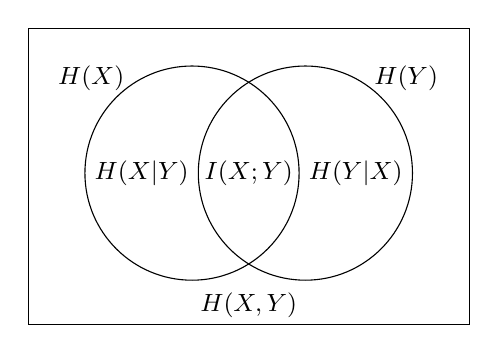
\begin{tikzpicture}[scale=0.8]
    \small
    % Labels
    \draw (0,0) node {$I(X;Y)$};
    \draw (-2.5,1.5) node {$H(X)$};
    \draw (2.5,1.5) node {$H(Y)$};
    \draw (-1.7,0) node {$H(X|Y)$};
    \draw (1.7,0) node {$H(Y|X)$};
    \draw (0,-2.1) node {$H(X,Y)$};
    % Circles
    \draw (-0.9,0) circle (1.7cm);
    \draw (0.9,0) circle (1.7cm);
    % Bounding Rectangle
    \draw (-3.5,-2.4) rectangle (3.5,2.3);
  \end{tikzpicture}
  \caption{Venn Diagram of Information-Theoretic Quantities}%
  \label{fig:venn-information}
\end{figure}

\subsection{Information-Theoretic View of GANs}%
\label{sec:info-value-function}%

We can now write a bit more about $\V = \mathbb{E}_{x \sim \pt}[{\log
  D_\theta(x)}] + \mathbb{E}_{z \sim \pz}[\log{(1 - D_\theta(G_\phi(z)))}]$ from
the perspective of information theory. The proposition presented below does not
consider the limiting behaviour of $D$ and $G$. Rather, we consider the
behaviour at each step of the algorithm. Section~\ref{sec:optimization-dynamics}
considers the limiting behaviour of the dynamics between $D$ and $G$.

We claim that the goal of GAN training is to minimize the Kullback-Leibler
divergence of the target probability distribution $\pt$ over the data and the
distribution of mass the discriminator $\D$ assigns to these data points.
Additionally, GAN training also maximizes the Kullback-Leibler divergence of the
generator's prior probability distribution $\pz$ and the distribution of mass
the discriminator assigns to synthetic data points $\D(\G(z))$. Lastly, GAN
training minimizes the Kullback-Leibler divergence of the generator's prior
distribution $\pz$ and the amount of mass the discriminator $\D(\G(z))$ assigns
to synthetic data points.

\begin{remark}
  The Kullback-Leibler divergence in this context can be thought of as how much
  more surprised we will be by outcomes drawn from $(\&X, p)$ since we are using
  an approximation $q$ of the true probability distribution $p$ over the set
  $\&X$.
\end{remark}

\begin{proposition}%
  \label{thm:info-objective}%
  If we consider
  \begin{align}
    \label{eq:consider}
    \min_\phi \max_\theta \mathbb{E}_{x \sim \pt}[{\log D_\theta(x)}] + \mathbb{E}_{z
    \sim \pz}[\log{(1 - D_\theta(G_\phi(z)))}]
  \end{align}
  from an information theoretic perspective, we can infer the training
  objectives of the GAN algorithm are to find
\begin{enumerate}[(i)]
  \item $\theta \in \Theta$ to minimize $\KL{\ptx}{\D(x)}$ and
    maximize $\KL{\pzz}{\D(\G(z))}$;
  \item $\phi \in \Phi$ to minimize $\KL{\pzz}{\D(\G(z))}$.
  \end{enumerate}
\end{proposition}

\begin{proof}
  The first term of $\V$ is the negative cross entropy of $\pt$ and
  the distribution induced by $\D(x)$,
\begin{align}
  \label{eq:neg-cross-entropy}
  - \&H(\pt, \D) = \sum_{x \in \&X}\ptx\log(\D(x)) = \mathbb{E}_{x \sim \pt} \left[\log(\D(x))\right].
\end{align}
Since we train the discriminator to maximize
(\ref{eq:neg-cross-entropy}) we can think of this as minimizing its
negative, which is equivalent to minimizing the cross entropy of $\pt$
and the distribution induced by $\D(x)$, which occurs when the
Kullback-Leibler divergence of $\pt$ and $\pd$ is 0, since
\begin{align}
  \&H(\pt,\D) & = - \sum_{x \in \&X} \ptx \log \pd \\
                   & = -\sum_{x \in \&X} \ptx \log \ptx + \sum_{x \in \&X} \ptx \log \ptx - \sum_{x \in \&X} \ptx \log \pd \\
                   & = -\sum_{x \in \&X} \ptx \log \ptx + \sum_{x \in \&X} \ptx \log {\ptx \over
                     \pd}  \\
                   & = H(\pt) + \KL{\pt}{\D}.
\end{align}
Since we do not touch $\pt$ during training, the only way to minimize
$\&H(\pt,\D)$ is to train $\D$ to minimize $\KL{\pt}{\D}$, which occurs when
$\pt = \D$. Therefore, when $\D$ has been optimized, $\D(x)$ will return the
probability that $x$ was sampled from $\pt$, which equals $\pt$ when $\D$ is
optimal. The second term of (\ref{eq:consider}),
\begin{align}
  \mathbb{E}_{z \sim \pz}\left[\log(1 - \D(\G(z)))\right] =
  \sum_{z \sim \pz} \pzz \log (1 - \D(\G(z)))
\end{align}
was maximized by $\D$, which is equivalent to $\D$ maximizing
\begin{align}
  -\sum_{z \sim \pz} \pzz \log (\D(\G(z))),
\end{align}
which is the cross entropy of $\pz$ and $\D(\G(z))$. This means $\D$ is trying
to make $\pz$ and $\D(\G(z))$ to be as different as possible. And given a fixed
discriminator $\D$, we train the $\G$ to minimize the same equation, which can
be expressed equivalently as minimizing
\begin{align}
  -\sum_{z \sim \pz} \pzz \log (\D(\G(z)))
\end{align}
the cross entropy of $\pz$ and $\D(\G(z))$.
\end{proof}

The interpretation of the above theorem is that the generator wants the
discriminator's decision on the generated data to be as uninformative as random
noise. The discriminator wants the distribution of its decision over the
training data to match the empirical probability distribution, while at the same
time, the discriminator wants its decision on the generated data to be more
informative than noise.

Next, we look at the optimization steps as the dynamics between approximating a
divergence and minimizing the same divergence.

\subsection{Optimization Dynamics}%
\label{sec:optimization-dynamics}

We discussed training $\D$ and $\G$ from the perspective of game theory in
Section~\ref{sec:derivation}. Now let us look at these results more rigorously
and with some actual calculations. Throughout this section, we will use the
following notation. Let $\&X$ be our data and $\pt$ the true probability
distribution over $\&X$. Let $\tilde{\&X}$ be the generated data and $\pg$ be
the distribution over $\tilde{\&X}$ induced by $\G$. Let $X$ be a random sample
from $(\&X, p^*)$, $\tilde{X}$ be a random sample from $(\tilde{\&X}, p_\phi)$,
and let $Z$ be a random sample from the prior probability space $(\&Z, \pz)$.

Throughout this section we will make use of not only
\begin{align}
  V(\phi, \theta)(X, Z) & = \sum_{x \in X}\pt\log{\D(x)} +
                          \sum_{z \in Z}\pz\log{(1 - \D(\G(z)))},
\end{align}
but of two equivalent variations as well. The first variation, $\tilde{V}(\phi,
\theta)(X, \tilde{X})$, is obtained by changing the second argument of $\V$ from
a sample of noise $Z$ to a sample from the generator $\G(Z) = \tilde{X}$. We
compute the second expectation with respect to $\pg$, i.e.\ we have
\begin{align}
  \tilde{V}(\phi, \theta)(X, \tilde{X}) = \sum_{x \in X}\ptx\log{\D(x)} + \sum_{\tilde{x} \in\tilde{X}}\pgx\log{(1 - \D(\tilde{x}))}.
\end{align}
For the second variation, $\&V$, we are going to embed our data into
$U \subset \R^2$, where each $u_i$ is associated with a pair
$(x_i, \tilde{x}_i)$. Then we can define the following function
\begin{align}
  \label{eq:joined}
  \Va(U) = \sum_{u \in U} \ptu \log \D(u) + \pgu \log(1 - \D(u)),
\end{align}
which we will use as short-hand for
\begin{align}
  \label{eq:joined-verbose}
  \sum_{u \in U} (p^* \circ \pi)(u)\log (\D \circ \pi)(u) + (\pg \circ \tilde{\pi})(u) \log(1 - (\D \circ \tilde{\pi})(u)),
\end{align}
where $\pi$ and $\tilde{\pi}$ are projections, i.e. $(f \circ \pi)(u) = (f
\circ \pi)((x, \tilde{x})) = f(x)$ and $(f \circ \tilde{\pi})(u) = (f
\circ \tilde{\pi})((x, \tilde{x})) = f(\tilde{x})$.

\begin{theorem}%
 \label{theorem:minimax}
 For any fixed $\G$, $\D$ maximizes $\V$ by playing its minimax
 decision rule and in doing so returns the following function
  \begin{align}
    \argmax_{\D}\V(\cdot) = \Dstar{\cdot}.
  \end{align}
\end{theorem}

\begin{proof}
  We compute the derivative of $\Va$ with respect to $\theta$,
  \begin{align}
    \label{eq:derivatives}
    {\partial \Va(U) \over \partial \theta} = \sum_{u \in U}\left[ \ptu { {\partial \D(u) \over \partial \theta} \over \D(u)} -
    \pgu {{\partial \D(u) \over \partial \theta} \over (1 - \D(u))}\right],
  \end{align}
  and when we let the derivative equal zero (looking only at the summand for
  clarity of notation) we can uncover $\D^*(u)$, by solving for $\D(u)$
  \begin{align}
    \label{eq:20}
    {\ptu \over \D(u)} = {\pgu \over (1 - \D(u))} \iff \D^*(u) = {\ptu \over \pgu + \ptu}.
  \end{align}
  Hence, for any fixed generator $G_\phi$, $\Va(U)$ is maximized when $\D$ takes
  the following action
  \begin{align}
    \label{eq:13}
    \D^*(u) = \Dstar{u}.
  \end{align}
  Hence $\argmax_{\D}\V(\cdot, \cdot) = \Dstar{\cdot}$.
\end{proof}

Now that we have the minimax decision rule, we can place it in the
value function $\tilde{V}$, to uncover
$\max_{\D}\tilde{V}(\phi, \theta)(X, \tilde{X})$, equal to
\begin{align}
  \label{eq:sum-of-two-kl-divergences}
   \mathbb{E}_{x \sim \pt}\left[\log{{\ptx \over p_{\phi}(x)+ \ptx}}\right] + \mathbb{E}_{\tilde{x} \sim \pg}\left[\log{\pgx \over \pgx + p^*(\tilde{x})} \right],
\end{align}
which is the sum of two Kullback-Leibler divergences (which is related
to the Jenson-Shannon divergence of $\pt$ and $\pg$)
i.e. $\max_{\D}\V(X, Z)$ is equal to
\begin{align}
  \label{eq:16}
  \KL{\pt}{p_{\phi} + \pt} + \KL{\pg}{\pg + p^*}.
\end{align}
\begin{lemma}
  The minimax value for $\D$, i.e. $\min_{\phi}\max_{\theta}\V(X, Z)$, is $ - \log{4}$.
\end{lemma}

\begin{proof}
  The training goal for $\G$ is to learn $\pt$, so the optimal $\G$ is $\G^* =
  \pt$. If this optimal $\G^*$ is place inside (\ref{eq:16}), we obtain
  \begin{align}
    \label{eq:side-note}
    V(\phi^*, \theta)(X, \tilde{X}) & = \sum_{x \in X}\ptx \log{\ptx \over 2 \ptx} + \sum_{\tilde{x} \in \tilde{X}}p^*(\tilde{x}) \log{ p^*(\tilde{x}) \over 2 p^*(\tilde{x})} \\
                      & = \sum_{x \in X} \ptx \log {1 \over 2} + \sum_{\tilde{x} \in \tilde{X}} p^*(\tilde{x}) \log {1 \over 2} \\
                      & = -\log{4}
  \end{align}
  Hence, the minimax value is $ - \log{4}$.
\end{proof}

\begin{theorem}%
  \label{thm:limiting}
  When $\D$ is optimal, minimizing $\V$ as a function of $\phi$ is equivalent to
  optimizing the Jensen-Shannon divergence.
\end{theorem}

\begin{proof}
  We can make the relationship between (\ref{eq:16}) and the
  Jensen-Shannon divergence by adding and subtracting $\log{4}$ from
  (\ref{eq:16}), which yields
  \begin{align}
    \label{eq:desired}
    V(\phi, \theta^*) = 2 \cdot \JSD{\pt}{\pg} - \log{4},
  \end{align}
  which is what we wanted. See Appendix~\ref{sec:proof-for-jsd-thing} for
  complete details.
\end{proof}

\subsection{Discussion}

% Theoretically, one reason that GANs are so successful is because
% they do not rely on traditional maximum likelihood methods, which
% are equivalent to minimizing the Kullback-Leibler divergence.

% To see this, let $p\left(x | \theta^{(*)}\right)$ be a probability
% distribution we wish to estimate and let
% $p\left(x | \theta^{\left(t\right)}\right)$ be our estimate at
% iteration $t$.  Then
% \begin{align}
%   \label{eq:equivalent-mle}
%   \KL{p\left(x | \theta^{(*)}\right)}{p\left(x | \theta^{\left(t\right)}\right)} =
%   H\left(p\left(x | \theta^{(*)}\right)\right) -
%   \mathbb{E}_{x \sim p\left(x | \theta\right)}\left[ \log p\left(x | \theta^{\left(t\right)}\right) \right],
%  \end{align}
% and minimizing the cross entropy term on the right is equivalent to maximizing
% \begin{align}
%   \mathbb{E}_{x \sim p\left(x | \theta\right)}\left[ \log p\left(x | \theta^{\left(t\right)}\right) \right].
% \end{align}
% Maximizing this term is equivalent to maximizing the likelihood
% function for $p\left(x | \theta\right)$.

% The discriminator's job is to classify data points as real or fake,
% which is equivalent to compression. The discriminator is optimized
% to cluster the data into two classes, real and fake. Neural networks
% are good at finding regularities in data and one way to express
% regularity is by clustering similar objects into groups.

This section included two information theoretic perspectives on GAN training.
Theorem~\ref{thm:limiting} considered the theoretical, limiting behaviour of
GANs and~\ref{thm:info-objective} considered what happens at each step of the
optimization.

As for Theorem~\ref{thm:limiting}, the measure that $G$ minimizes changes at
each training step since $D$ forces $\V$ into a better approximation of the
Jensen-Shannon divergence one step at a time by performing the actions
enumerated in Theorem~\ref{thm:info-objective}. It is useful to consider what
happens at each step of training. When we do that, we observe the generator and
discriminator minimizing and maximizing the Kullback-Leibler divergence to
optimize the fit of $D$ and $G$ to $(\&X, \pt)$.

%%% Local Variables:
%%% mode: latex
%%% TeX-master: "../thesis.tex"
%%% End:

% Optimal Transport Chapter
\section{Optimal Transport}%
\label{sec:optimal-transport}

\vspace{1cm}

\begin{figure}[h]%
  \label{fig:paradise}
  \centering
  \fcolorbox{black}{white} {
    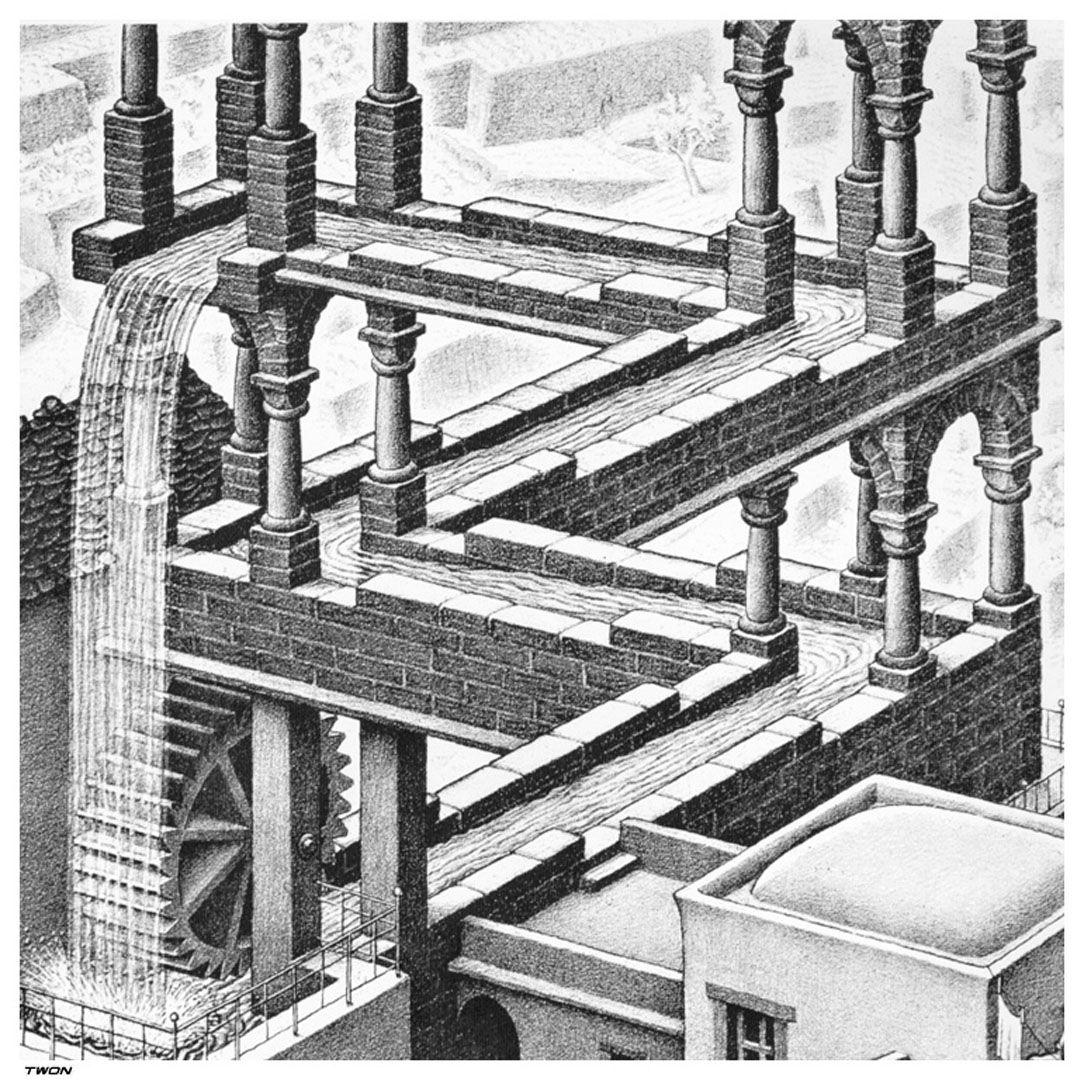
\includegraphics[width=0.3\textwidth]{escher}
  }
  \caption{M.C. Escher, ``Waterfall'', 1961.}
\end{figure}

\vspace{1cm}

\lettrine[lines=3]{\Royal~S}{ection~\ref{sec:information-theory}
  uncovered how the generator minimizes} an approximation of the
Jensen-Shannon divergence of $\pt$ and $\pg$ which the discriminator
approximated at each training step.

In this section we discuss the limitations of $\V$ as the GAN
objective function which come from the metric topology induced by the
Jensen-Shannon divergence. To this end, we provide an introduction to
some relevant concepts from topology in order to understand the
aforementioned limitations.

We also provide an introduction to optimal transport and what is
commonly referred to as the earth mover or Wasserstein distance in
order to properly cover a variant of the GAN algorithm called the
Wasserstein GAN (WGAN). The WGAN was introduced
by~\cite{ref:arjovsky-2017} from the Courant Institute of Mathematical
Sciences as an attempt to overcome certain obstacles in GAN training.

The moral of this section is the choice of distance function to
furnish a space $\&X$ with has profound consequences on properties of
continuity and therefore the ability of sequences of probability
distributions to convergence within $\&X$.

% The reason for this has to do with the topological properties
% induced by the choice of distance.

A topological space is the most general notion of a mathematical space
that allows for the definition of concepts like continuity and
convergence.  Other spaces such as manifolds and metric spaces are
specializations of topological spaces with extra structure or
constraints.  A space $\&X$ can be furnished with various different
distance functions.  The \textit{open balls} form the base for a
topology on $\&X$, which makes $\&X$ into a \textit{topological
  space}.

% \begin{definition}
%   Let $(\&X, d)$ be a metric space. An \textbf{open ball} of radius
%   $r \in \R^+$ around the point $x_0 \in \&X$ is the set
%   \begin{align}
%     \&B_r(x_0) = \left\{ x \in \&X : d(x,x_0) < r \right\}.
%   \end{align}
%   That is to say $\&B_r(x_0)$ is the set of all points in $\&X$ that
%   are not more than a distance of $r$ from $x_0$.
% \end{definition}

\begin{definition}%
  \label{def:topology1}
  Let $\&X$ be any set. A \textbf{topology} $\&T$ on $\&X$ is a
  collection of subsets of $\&X$, each called an open set, such that
  \begin{enumerate}[(i)]
  \item the empty set and the set containing all of $\&X$ are open;
  \item the intersection of finitely many open sets is an open set;
  \item the union of any collection of open sets is an open set.
  \end{enumerate} The set $\&X$ along with a topology $\&T$ on $\&X$
  is called a \textbf{topological space}.
\end{definition}

The notion of the \textit{open ball} is fundamental to the topology of
a metric space.  Useful topological definitions (useful from the
perspective of the practising statistician) can be formed from the
notion of the \textit{open ball}.

\begin{definition}%
  \label{def:open-ball}
  Let $(\&X, \&D)$ be a metric space. An \textbf{open ball} of radius
  $r \in \R^+$ around the point $x_0 \in \&X$ is the set
  \begin{align}
    \&B_r(x_0) = \left\{ x \in \&X : \&D(x,x_0) < r \right\}.
  \end{align}
  That is to say $\&B_r(x_0)$ is the set of all points in $\&X$ that
  are within $r$ distance from $x_0$.
\end{definition}

\begin{definition}%
  \label{def:topology2}
  Let $(\&X, d)$ be a metric space.  The topology generated by the
  basis of open balls
  $\&B = \{\&B_d(x, \epsilon) \mid x \in \&X, \epsilon > 0\}$ is
  called the \textbf{topology induced by} $d$ and is referred to as a
  \textbf{metric topology}.
\end{definition}

Different metrics induce different topologies which are characterized
by the quality of granularity.

\begin{theorem}%
  \label{thm:granularity}
  Let $d$ and $d^\prime$ be metrics on a set $\&X$, and let $\&T$ and
  $\&T^\prime$, be the respective topologies they induce.
  $\&T^\prime$ is \textbf{finer} than $\&T$ if and only if for each
  $x \in \&X$ and $\epsilon > 0$, there exists a $\delta > 0$ such
  that $\&B_{d^\prime}(x, \delta) \subset \&B_d(x, \epsilon)$.
\end{theorem}

\begin{definition}%
  \label{def:convergence-metric-space}
  Let $\&X$ be any finite set of events, and $\&P$ be the space of all
  probability distributions over $\&X$ with equal support. Let
  $d: \&P \times \&P \mapsto \mathbb{R}$ be a metric on this space.  A
  sequence of probability distributions ${(P_n)}_{n \in \mathbb{N}}$
  \textbf{converges} to a probability distribution $P$ if for any
  $\epsilon > 0$ there exists $N(\epsilon) \in \mathbb{N}$ such that
  $d(P_n,P) < \epsilon$ for all $n > N(\epsilon)$.
\end{definition}

The ease in which a sequence of probability distributions
${(P_n)}_{n \in \mathbb{N}}$ converges to some $P$ is determined by
the notion of distance.  The Kullback-Leibler and Jensen-Shannon
divergences induce a coarser topology than the topology induced by the
\textit{earth mover distance}. The interested reader can see the proof
of this in~\cite{ref:arjovsky-2017}.  To ease convergence, we want to
place a finer topology on $\&P \times \&P$.  A finer topology means we
can pack more open sets over $\&P \times \&P$, which makes it easier
to define a \textit{continuous map} from $\&P \times \&P$ to $\R^+$.
If a metric $d$ induces a finer topology on a space than another
metric $d^\prime$, then we say $d$ is a weaker notion of distance than
$d^\prime$.

We can think of continuity and convergence in more than one way, below
we include the relevant definitions from both the topological and
metric space points of view.

\begin{definition}%
  \label{def:continuity-metric-space}
  A function $f: \R \mapsto \R$ is \textbf{continuous} if for every
  $x_0 \in \R$, $\epsilon > 0$, there exists $\delta > 0$ such that if
  $|x - x_0| < \delta$, then $|f(x) - f(x_0)| < \epsilon$.
\end{definition}

Continuous functions between topological spaces preserve proximity,
i.e.\ a continuous function maps points that are close together in one
space to points that are close together in the other space.

\begin{definition}%
  \label{def:convergence-topological-space}
  In a topological space $(\&X, \&T)$, a sequence of points
  \textbf{converges} to $x \in \&X$ if for every neighborhood $U$ of
  $x$, there is an $N \in \mathbb{N}$ such that $x_n \in U$ for all
  $n \geq N$.
\end{definition}

The following is the topological definition of continuity. Briefly,
$f$ is continuous if the \textit{preimage} of every open set is open.

\begin{definition}%
  \label{def:pre-image}
  Given a function $f: \&X \mapsto \&Y$ and a point $y \in \&Y$,
  define $f^{-1}(y)$, the \textbf{preimage} of $y$, to be the set
  $\{x \in \&*X \mid f(x) = y\}$.  For any set $A \subset \&Y$, the
  preimage of $A$, $f^{-1}(A) = \{x \in \&X \mid f(x) \in A\}$.
\end{definition}

\begin{definition}%
  \label{def:continuity-topological-space}
  Let $\&X$ and $\&X^\prime$ be topological spaces. A function
  $f: \&X \mapsto \&X^\prime$ is \textbf{continuous} if $f^{-1}(V)$ is
  open in $\&X$ for every open set $V$ in $\&X^\prime$.
\end{definition}

The problem with the Kullback-Leibler and Jensen-Shannon divergences
is that they are strong notions of distance. Which means continuity of
the loss function may be lost under certain commonly encountered
circumstances in GAN training.

\subsection{Limitations of the Kullback-Leibler Divergence}

In~\cite{ref:arjovsky-2017}, the authors use the example of learning
parallel lines and here we present the same example. This is an
example of what happens with the Kullback-Leibler and Jensen-Shannon
divergences when we compare distributions over the same space but with
disjoint supports, see Definition \ref{def:kl-divergence} for more
information on the Kullback-Leibler divergence.

\begin{example}[Learning Parallel Lines]
  \begin{figure}[h] \centering
    \begin{tikzpicture}[scale=2,>=stealth]
      \draw[line] (-1,-0.5) rectangle (2,2);
      \draw[red, thick, ->] (0,0) -- (0,1);
      \draw[blue, thick, ->] (1,0) -- (1,1);
      \draw[dotted] (-0.8,0) -- (1.8,0) node[anchor=north east]{$x$};
      \draw[dotted] (0,-0.3) -- (0,1.8) node[anchor=north east]{$y$};
      \draw (0,0) node[anchor=north east]{$(0,z)$};
      \draw (1,0) node[anchor=north east]{$(\phi,z)$};
    \end{tikzpicture}
    \caption{Parallel Lines}%
    \label{fig:parallel-lines}
  \end{figure}%
  \label{example:learning-parallel-lines}

  Let $\&X = \R^2$ and let $p_0(z)$ be the distribution of tuples
  $(0, z) \subset \R^2, z \in [0, 1]$, i.e.\ we have a uniform
  distribution over the $y$-axis of $\R^2$ of length 1 starting at the
  origin. Let $\G(z)$ be the distribution of tuples
  $(\phi, z) \subset \R^2$ (a generative model), where $\phi$
  parameterizes the location of the distribution with respect to the
  $x$-axis. We want to train $\G(z)$ to approximate $p_0(z)$, i.e.\ we
  want $\phi \to 0$.
  \begin{enumerate}[(i)]
  \item If we use the Kullback-Leibler divergence to measure the
    distance between $p_0(z)$ and $\G(z)$ we observe the following
    discontinuity between changes in the parameter $\phi$ and the
    divergence
    \begin{align}
      \KL{p_0(z)}{\G(z)} = \E{z \sim p_0(z)}{\log{p_0(z)\over\G(z)}},
    \end{align}
    since the expectation above is taken with respect to the
    distribution over the line $(0, z)$, the line will have measure
    zero with respect to the distribution $\G(z)$. Thus
    $\KL{p_0(z)}{\G(z)} = \infty$, unless $\phi = 0$, then
    $\KL{p_0(z)}{\G(z)} = 0$. The same occurs with
    $\KL{\G(z)}{p_0(z)}$.
  \item The Jensen-Shannon divergence ends up being equally useless
    since
    \begin{align}
      \JSD{p_0(z)}{\G(z)} & = {1 \over 2} \E{z \sim p_0(z)}{\log{p_0(z)
                            \over p_m(z)}} + {1 \over 2} \E{z \sim
                            \G(z)}{\log{\G(z) \over p_m(z)}} \\
                          & = {1 \over 2} \E{z \sim p_0(z)}{\log{2}} + {1
                            \over 2} \E{z \sim \G(z)}{\log{2}} \\
                          & = \log{2},
    \end{align}
    where $p_m(z) = {p_0(z) + \G(z) \over 2}$. In the first term
    $\G(z) = 0$ because $z \sim p_0(z)$ and in the second term
    $p_0(z) = 0$ because $z \sim \G(z)$. Which is to say
    $\JSD{p_0(z)}{\G(z)} = \log{2}$, unless $\phi = 0$, in that case
    $\JSD{p_0(z)}{\G(z)} = 0$.
  \end{enumerate}
\end{example}

% The reason why this happens has something to do with topology. We
% need to relax the convergence requirements, we need to relax the
% continuity requirements.

The reason why this happens is a central topic
in~\cite{ref:arjovsky-towards-2017} and is due to the combination of
the strong notion of distance of the Jensen-Shannon divergence and the
artificially high dimensionality of most data sets.  For example, a
data set may live in $\R^n$ for some large $n$, but there may only be
variation of interest in a small number of dimensions. This is one of
the ideas motivating dimensionality reduction algorithms like PCA and
manifold learning algorithms in particular like
Isomap~\cite{ref:tenenbaum-2000}.

GANs are often used in the generation of realistic looking images. If
we consider an image to be a point in
$\&X = {[0, 255]}^{3 \times H \times W}$, the space of 8-bit RGB
images, and if we were to sample a point from this space, it would
most likely look like noise. Thus, any data set of images would
correspond to a very small subset, or \textit{data manifold}, of
$\&X$. An informal definition of a \textit{manifold} is more useful to
our discussion than a formal one. When we say \textbf{manifold}, we
mean a continuous geometrical structure with finite dimension (e.g.\ a
line, a curve, a plane, a surface etc\dots) embedded inside a space of
higher dimension than the manifold itself.  Locally, manifolds
resemble $\R^n$ for some $n$, i.e.\ they are locally flat.

Richard E. Bellman coined the term \textit{the curse of
  dimensionality}, to refer to the fact that when the dimensionality
of the data increases, the volume of the space scales at an
exponential rate and consequently data become effectively sparse. For
instance $10$ points can be evenly arrange along the unit interval
with $0.1$ units of distance between them. If we want to cover the
unit square with points $0.1$ units of distance apart, we would need
$100$ points; for the unit cube? 1000 points. Each time we add a
dimension, we need (in our case) 10 times as many points. Since the
space of all $L \times W$ 8-bit RGB images is very large, we get the
idea that even ``large'' image data sets are effectively small.

In the case of the GAN algorithm, it is unlikely that the generator
will generate points that are from the same data manifold that the
true data lie in. Which means $\pg$ and $\pt$ are likely to be
supported by disjoint lower dimensional manifolds and
$\KL{\pg}{\pt} = 0$, when the distributions are not equal, or
$\KL{\pg}{\pt} = \infty$.

% Concretely, issues arises with
% (\ref{eq:the-original-objective-function}) if $\forall \tilde{\*x}$,
% $(p^*(\tilde{\*x}) = 0)$ and if $\forall \*x$, $(\pg(\*x) = 0)$ we
% end up with $\max_{\D}\*V(\*X, \widetilde{\*X}) = 0$. This issue may
% arise if the supports of $\pt$ and $\pg$ lie in disjoint
% \textit{submanifolds} of $\&X$.

\subsubsection*{Perfect Discriminator}

The goal of GAN training is to optimize $\D$ until it converges to
$\D^*$ forcing (\ref{eq:the-original-objective-function}) into a
function related to the Jensen-Shannon divergence.  $\G$ is then
optimized to minimize this divergence, but in practice $\D$ very
quickly converges to be what~\cite{ref:arjovsky-towards-2017} call a
\textit{perfect discriminator}.

\begin{definition}%
  \label{def:perfect-discriminator}
  A \textbf{perfect discriminator} is a function $D:
  \&X \mapsto [0,1]$ that has accuracy 1 for all $\*x$ in the supports
  of $\pt$ and $\pg$. In other words
  \begin{align}
    \mathbb{P}_{\&X}(\{\{\*x \in \&X : \pt > 0\} : D(\*x) = 1 \} )= 1, \\
    \mathbb{P}_{\tilde{\&X}}(\{\{\tilde{\*x} \in \tilde{\&X} : \pg > 0\} : D(\tilde{\*x}) = 0 \} )= 1.
  \end{align}
\end{definition}

\begin{theorem}%
  \label{thm:perfect-discriminator}
  If $\D$ is a perfect discriminator, then $\D$ is constant on both
  supports of $\pg$ and $\pt$ and $\nabla{V_\phi} = 0$, which means
  the gradient updates provide $\G$ no amount of movement in the
  $\phi$-parameter space.
\end{theorem}

\begin{proof}%
  \label{prf:perfect-discriminator}
  Let $\alpha > 0$ denote the learning-rate parameter and when we
  write $\G \gets \dots$ we mean the parameters $\phi$ are replaced
  with the output of the calculation on the right-hand side of the
  assignment operator. Then
  \begin{align}
    \label{eq:g-updates-no-good}
    \G^{(t+1)} & \gets \G^{(t)} - \alpha\nabla_\phi {1 \over m} \sum_{i=1}^m \log\left( 1 - \D^{(t+1)}(\G^{(t)}(\*z_i)) \right) \\
    \implies \G^{(t+1)} & \gets \G^{(t)} - \alpha\nabla_\phi {1 \over m} \sum_{i=1}^m \log{ \left( 1 - \D^{(t+1)}(\tilde{\*x}_i) \right)} \\
    \implies \G^{(t+1)} & \gets \G^{(t)} - \alpha\nabla_\phi {1 \over m} \sum_{i=1}^m \log{1} \\
    \implies \G^{(t+1)} & \gets \G^{(t)}
  \end{align} which is to say, $\G$ does not get updated.
\end{proof}

\begin{theorem}%
  \label{thm:too-early}
  If $\D$ converges to a perfect discriminator too early in training,
  and $\G$ has stopped learning, then $\D$ will not learn anything
  from the gradient updates.
\end{theorem}

\begin{proof}
  \begin{align}
    \label{eq:d-updates-no-good}
    \D^{(t+1)} & \gets \D^{(t)} - \alpha \nabla_\theta {1 \over m}
                 \sum_{i=1}^n \left( \log D^{(t)}_\theta(\mathbf{x}_i)
                 + \log{(1 - D^{(t)}_\theta(G^{(t)}_\phi(\mathbf{z}_i)))} \right) \\
    \implies \D^{(t+1)} & \gets \D^{(t)} - \alpha\nabla_\theta {1 \over m} \sum_{i=1}^n \left( \log{1} + \log{1} \right) \\
    \implies \D^{(t+1)} & \gets \D^{(t)}
  \end{align} which is to say, $\D$ does not get updated.
\end{proof}

Even though $\D$ is a perfect discriminator, it is only good at
telling apart obviously different distributions. This begets the need
for a ``gentler'' discriminator.  The WGAN paper tackles the issues
mentioned above by using a different objective function and training
routine.  It is interesting to look into the history of the
Wasserstein distance and we will see that the WGAN is a modern
implementation to an old transportation problem.

\subsection{The Monge-Kantorovich Transportation Problem}

Convergence issues that arise from the original GAN formulation have
inspired novel takes on GAN training and implementation. One
influential variation, inspired by \textit{optimal transport theory},
is the Wasserstein GAN~\cite{ref:arjovsky-2017}. Before we introduce
the Wasserstein GAN, it will be informative to introduce optimal
transport theory.

The Wasserstein GAN is named after the Wasserstein-1 distance,
otherwise known as the \textit{earth mover distance}. The distance in
question however, was not discovered by Leonid Wasserstein, rather it
was discovered by the work of Gaspard Monge and Leonid
Kantorovich. Wasserstein did publish a paper with a definition of the
distance in 1969, but he did not discover it.

Gaspard Monge (1746~\textendash~1818) was a mathematician, physicist,
and founder and head of the \'Ecole Polytechnique, located just
outside of Paris. In 1781 he formulated the transportation problem
\textit{Excavation and Embankments}, which was about how to transport
soil during the construction of forts and roads with minimal
transportation cost.

Leonid Kantorovich (1912~\textendash~1986) is regarded as one of the
founders of mathematical economics and received a Nobel prize in 1975
for his contributions.  He also established the theory of linear
programming in 1938. In 1939 Kantorovich published a booklet
\textit{Mathematical Methods of Organizing and Planning of
  Production}, and later he wrote brief paper called \textit{On
  Translocation of Masses} in 1942.

In 1947 Kantorovich read the proceedings to a public session dedicated
to Monge. The proceedings contained the transcript of a talk about
Monge's transportation problem. When Kantorovich read the problem, he
saw how it related to his own work and it was then that the
transportation problem became known as the Monge-Kantorovich
transportation problem.

The following is the definition of a transport plan as defined by
Kantorovich in 1942~\cite{ref:kantorovich-1942}~and can be found
in~\cite{ref:vershik-2013}.

\begin{definition}%
  \label{def:transport-plan}
  Let $\&X$ be any space. A \textbf{transport plan} is a probability
  measure $\gamma(x, y)$ on $\&X \times \&X$, whose projection
  $(\gamma(x, y) \circ \pi_{x}) = P$ and whose projection
  $(\gamma(x, y) \circ \pi_{y}) = Q$ i.e.\ the marginal distributions
  of $\gamma(x, y)$ with respect to $x$ and $y$, are the measures $P$
  and $Q$.
\end{definition}

\begin{remark}%
  \label{rmrk:mass}
  Each joint distribution $\gamma(x, y)$ represents the amount of mass
  needed to be move from each $x$ to each corresponding $y$ in order
  to transform $P$ into $Q$.
\end{remark}

\begin{definition}%
  \label{def:transport-cost}
  The \textbf{transport cost} for a given transport plan is given by
  \begin{align}%
    \label{eq:expected-work}
    \left(\int_{\&X}\int_{\&Y}||x-y||^p\gamma(x, y)dxdy \right)^{1 \over p}
  \end{align}
  The distance the mass needs to travel $||x-y||^p$ multiplied by the
  amount of mass $\gamma(x, y)$ gives the expected amount of work
  required to transform $P$ into $Q$.
\end{definition}

Now the goal of optimal transport is to find the transport plan with
the minimal cost, thus we wish to find
\begin{align}%
  \label{eq:min-work}
  \&W_p(P, Q) = \inf_{\gamma(x,y) \in \Gamma(x,y)} \left( \int_{\&X}\int_{\&Y}||x-y||^p\gamma(x, y)dxdy \right)^{1 \over p}
\end{align}
where $p \geq 1$. For $p = 1$ we call $\&W_1(P, Q)$ the Wasserstein
distance. This is what is used in the Wasserstein GAN. The algorithm
in (\ref{eq:min-work}) can be stated more succinctly as
\begin{align}
  \label{def:w1-wgan}
  \&W_1(P, Q) = \inf_{\gamma(x, y) \in \Gamma(x,y)}\mathbb{E}_{(x,y) \sim \gamma(x, y)} \left[ || x-y || \right]
\end{align}
\begin{remark}
  The definition given above in (\ref{def:w1-wgan}) involves an
  intractable infimum (it's not computationally feasible to find the
  infimum over all possible $\gamma(x, y)$).
\end{remark}

\subsection{The Wasserstein GAN}

The distance given in (\ref{def:w1-wgan}) does not yet improve
anything given the intractability of the infimum. However, the
following theorem, attributed to Kantorovich and his student
Rubinstein, saves the day.

\begin{definition}
  Let $(\&X, \&D_\&X)$ and $(\&Y, \&D_\&Y)$ be two metric spaces and
  let $f: \&X \times \&Y \mapsto \R$ be a real-valued function mapping
  elements from $\&X$ to $\&Y$. A \textbf{K-Lipshitz} function is
  defined as
  \begin{align}
    \label{eq:lip1}
    \&D_{\mathcal{Y}}(f(x_1), f(x_2)) \leq K \cdot {\&D}_{\mathcal{X}}(x_1, x_2)
  \end{align}
  for all $x_1$ and $x_2 \in \&X$. (\ref{eq:lip1}) can be stated as
  \begin{align}
    {\&D_{\mathcal{Y}}(f(x_1), f(x_2)) \over \&D_{\mathcal{X}}(x_1, x_2)} \leq K,
  \end{align}
  which is to say the rate of change of $f$ is bounded above by the
  Lipshitz constant $K$.
\end{definition}

\begin{theorem} The \textit{Kantorovich-Rubinstein duality} says
  \begin{align}
    \inf_{\gamma \in \Gamma(\mathbb{P}_r,
    \mathbb{P}_g)}\mathbb{E}_{(x,y) \sim \gamma(x, y)} \left[ || x-y
    || \right]
  \end{align}
  is equivalent to
  \begin{align} \sup_{f \in \&{F}} \mathbb{E}_{x \sim \pt}\left[ f(x)
    \right] - \mathbb{E}_{\tilde{x} \sim \pg}\left[ f(\tilde{x}) \right]
  \end{align}
  where $f(x) - f(y) \leq ||x-y||$ and $\&{F}$ is the set of all
  1-Lipshitz functions.
\end{theorem}

The topology induced by the Kullback-Leibler divergence is much
coarser than the topology induced by the Kantorovich-Rubinstein
distance, which is a weak enough notion of distance to relax
convergence requirements. See~\cite{ref:villani-2008} for more
information on the Kantorovich-Rubinstein distance.

\begin{example}[Learning Parallel Lines (Revisited)]
  When we use the Kantorovich-Rubinstein distance in the parallel
  lines problem.
  \begin{align}
    \&W_1(\G(z), p_0(z)) & = \inf_{\gamma \in
                           \Gamma(\G(z),p_0(z))}\mathbb{E}_{(x,y) \sim
                           \gamma(x, y)} \left[ || x-y || \right] \\
                         & =\inf_{\gamma \in \Gamma(\G(z),
                           p_0(z))}\mathbb{E}_{(x,y) \sim \gamma(x,
                           y)} \left[ \sqrt{(\phi - 0)^2 + {(z - z)}^2}
                           \right] \\
                         & =|\phi|
  \end{align}
\end{example}

The Kantorovich-Rubinstein distance provides a continuous measure of
distance even for probability distributions with disjoint supports.

\subsubsection*{The Wasserstein GAN Algorithm}

The following is the WGAN algorithm as presented in
\cite{ref:arjovsky-2017}.

\begin{figure}[H]
  \centering
  \begin{minipage}{\linewidth}
    \begin{algorithm}[H]
      Let $\epsilon > 0$ \textit{be the learning rate.} \\
      Let $c > 0$ \textit{be the clipping parameter.} \\
      Let $T > 0$ \textit{be the number of training iterations.} \\
      Let $K > 0$ \textit{be the number of training iterations for the
        critic.} \\
      Let $f_\theta: \Theta \times \&X \mapsto [0, 1]$ \\
      Let $\G: \Phi \times \&Z \mapsto \&X$ \\
      \For%
      {$t \in \{0, \dots, T\}$} {
        \For%
        {$k \in \{0, \dots, K\}$} {
          Let
          $\*Z = \{\*z_1, \dots, \*z_m\}$, \textit{where each
            $\*z_i$ is sampled according to $\pz$, the prior
            probability distribution over $\&Z$.  This batch will be
            used in the optimization of
            $\D$.} \\
          Let
          $\*X = \{\*x_1, \dots, \*x_m\}$, \textit{where each
            $\*x_i$ is from the training data.} \\
          Let
          ${\partial{V} \over \partial{\theta}} = \nabla_\theta\left[
            {1 \over m} \sum_{i=1}^m f_{\theta}(x_i) - {1 \over m}
            \sum_{i=1}^m f_{\theta}(\G(z_i))\right]$. \\
          Let
          $\theta \gets \theta + \epsilon \cdot \text{RMSProp}(\theta,
          {\partial{V} \over \partial{\theta}})$. \\

          Let $\theta \gets \text{clip}(\theta, -c, c)$.
        }

        Let $\*Z = \{\*z_1, \dots, \*z_m\}$, \textit{we sample a new
          batch according to $\pz$. This batch will be used in the
          optimization of
          $\G$.} \\

        Let
        ${\partial{V} \over \partial{\phi}} = - \nabla_\phi{1 \over m}
        \sum_{i=1}^m f_{\theta}(\G(z_i)).$ \\

        Let
        $\phi \gets \phi + \epsilon \cdot \text{RMSProp}(\phi,
        {\partial{V} \over \partial{\phi}}).$ \\
      }
      \caption{WGAN}
      \label{algo:wgawgann-algo}
    \end{algorithm}
  \end{minipage}
\end{figure}

\subsection{Discussion}
\textcolor{red}{TODO:}

The objective function inherits the strong topology from the
Jensen-Shannon and Kullback-Leibler divergences, hence Arjovsky has
refit an old solution to a new problem. The weaker notion of distance
provided by the earth mover distance provides a continuous objective
function.

When we defined the earth mover distance and the duality theorem, we
said that the sup was taken over the space of all 1-lipshitz
the way this was achieved in arjovky's paper was to clip the weight
parameters, which effectively reduced the amount the parameters can
change with each update.

%%% Local Variables:
%%% mode: latex
%%% TeX-master: "../thesis.tex"
%%% End:

% Conclusion
\section{Conclusion}

In Section \ref{sec:game-theory} we looked at game theory and how the
GAN algorithm can be cast as a game between two competing neural
networks.  The minimax strategy for $D$ was $D(x) = {1 \over 2}$ for
all $x$, which, if attained, would make it impossible for the
generator to minimize the value function, since $G$'s actions would no
longer affect the actions of $D$.  This strategy makes sense for $D$,
since it's the best anyone can do when confronted with maximum
uncertainty.

Section \ref{sec:information-theory} included two information
perspectives on GAN training. Theorem \ref{thm:limiting} considered
the theoretical, limiting behaviour of GANs and
\ref{thm:info-objective} considered what happens at each step of the
optimization.  This is similar to a macroscopic and microscopic view
of GAN training.

Section \ref{sec:optimal-transport} introduced optimal transport and
showed how the GAN algorithm has benefited greatly from the
application of the Kantorovich-Rubinstein distance from optimal
transport.  It takes a great deal of theoretical understanding to
build the a well-functioning learning system.  By recasting the GAN
algorithm as an optimal transport problem, \cite{ref:arjovsky-2017}
have put GANs on a solid theoretical foundation.

%%% Local Variables:
%%% mode: latex
%%% TeX-master: "../thesis"
%%% End:

\section*{Addendum: Advances in Generative Models (2019-2025)}

\subsection*{Introduction}

Since the completion of this thesis in 2019, the field of generative models has undergone revolutionary changes. While GANs continue to be influential, new paradigms have emerged that have transformed the landscape of generative AI. This addendum provides an overview of the most significant developments from 2019 to 2025.

\subsection*{The Rise of Diffusion Models}

The most significant development has been the ascendancy of diffusion models as the dominant paradigm for generative modeling.

\subsubsection*{Denoising Diffusion Probabilistic Models (DDPM)}
In 2020, Ho et al. introduced DDPMs, which simplified the diffusion process and achieved remarkable image generation quality. Unlike GANs, diffusion models are trained by gradually adding noise to data and then learning to reverse this process.

\subsubsection*{Latent Diffusion Models}
Rombach et al. (2022) introduced latent diffusion models, which operate in a compressed latent space rather than pixel space. This approach dramatically improved computational efficiency and enabled high-resolution image generation.

\subsubsection*{Stable Diffusion}
The release of Stable Diffusion in 2022 by Rombach et al. democratized access to high-quality image generation. Its open-source nature and efficiency made it widely adopted, leading to an explosion of applications.

\subsection*{Large-Scale Text-to-Image Models}

\subsubsection*{DALL-E 2 and 3}
OpenAI's DALL-E 2 (2022) and DALL-E 3 (2023) demonstrated unprecedented text-to-image generation capabilities, using a combination of diffusion models and CLIP-based text understanding.

\subsubsection*{Midjourney}
Midjourney, released in 2022 and continuously improved, became known for its artistic image generation capabilities and became a cultural phenomenon.

\subsubsection*{Google's Imagen and Parti}
Google introduced Imagen (2022) and Parti (2022), which pushed the boundaries of photorealistic image generation and text understanding.

\subsection*{Video Generation}

\subsubsection*{Make-A-Video}
Meta's Make-A-Video (2022) extended text-to-image generation to video, using diffusion models to generate short video clips from text prompts.

\subsubsection*{Sora}
OpenAI's Sora (2024) represented a major breakthrough in video generation, capable of generating minute-long videos with remarkable coherence and realism.

\subsection*{3D and Multimodal Generation}

\subsubsection*{3D Generation}
Models like DreamFusion (2022) and Magic3D (2023) enabled text-to-3D generation by extending diffusion models to 3D spaces.

\subsubsection*{Multimodal Models}
GPT-4 (2023) and Gemini (2023) demonstrated the power of multimodal models that can generate and understand text, images, audio, and video in a unified framework.

\subsection*{Theoretical Advances}

\subsubsection*{Score-Based Generative Modeling}
Song and Ermon (2019-2021) developed a unified framework connecting diffusion models, score-based generative models, and energy-based models, providing theoretical foundations for the success of diffusion models.

\subsubsection*{Flow Matching}
Lipman et al. (2023) introduced flow matching, a simpler and more flexible approach to generative modeling that has shown promise as an alternative to diffusion models.

\subsubsection*{Consistency Models}
Song et al. (2023) developed consistency models, which can generate samples in a single step, addressing the computational inefficiency of iterative sampling in diffusion models.

\subsection*{GANs in the New Era}

While diffusion models have dominated, GANs have continued to evolve:

\subsubsection*{StyleGAN Series}
StyleGAN2 (2020) and StyleGAN3 (2021) by Karras et al. continued to push the boundaries of GAN-based image generation, particularly for face synthesis.

\subsubsection*{GANs for Video}
Models like MoCoGAN (2023) and VideoGAN (2024) have adapted GANs for video generation tasks.

\subsubsection*{Conditional and Controllable Generation}
Research has focused on making GANs more controllable and interpretable, with applications in medical imaging, design, and content creation.

\subsection*{Efficiency and Scalability}

\subsubsection*{Knowledge Distillation}
Techniques for distilling large diffusion models into smaller, faster models have become crucial for practical applications.

\subsubsection*{Few-Shot and Zero-Shot Learning}
Models like DALL-E Mini (2022) and Stable Diffusion XL (2023) have demonstrated impressive few-shot and zero-shot generation capabilities.

\subsection*{Societal Impact and Challenges}

\subsubsection*{Deepfakes and Misinformation}
The improved quality of generative models has raised concerns about deepfakes and misinformation, leading to research in detection and watermarking techniques.

\subsubsection*{Copyright and Legal Issues}
The training of generative models on copyrighted data has led to legal challenges and debates about fair use and data rights.

\subsubsection*{Bias and Fairness}
Research has focused on understanding and mitigating biases in generative models, which can amplify societal biases present in training data.

\subsection*{Applications and Industry Adoption}

\subsubsection*{Creative Industries}
Generative models have been widely adopted in creative industries for content creation, design, and entertainment.

\subsubsection*{Healthcare}
Applications in medical imaging, drug discovery, and synthetic data generation have shown significant promise.

\subsubsection*{Scientific Research}
Generative models have been applied to scientific problems, including protein structure prediction, material design, and climate modeling.

\subsection*{Future Directions}

\subsubsection*{Multimodal and Interactive Generation}
Future research is likely to focus on more sophisticated multimodal generation and interactive systems that can respond to user feedback in real-time.

\subsubsection*{3D and Video Generation}
Improvements in 3D and video generation quality and efficiency are active areas of research.

\subsubsection*{Theoretical Understanding}
Despite empirical success, the theoretical understanding of diffusion models and large-scale generative models remains incomplete, presenting opportunities for future research.

\subsection*{Conclusion}

The period from 2019 to 2025 has seen generative AI transition from a research curiosity to a transformative technology with widespread applications. While GANs laid important foundations, diffusion models and large-scale multimodal systems have become the dominant paradigms. The field continues to evolve rapidly, with ongoing research addressing efficiency, controllability, theoretical understanding, and societal impact.

\subsection*{Key References (2019-2025)}
\begin{itemize}
    \item Ho, J., Jain, A.,\& Abbeel, P. (2020). Denoising Diffusion Probabilistic Models. NeurIPS.
    \item Rombach, R., Blattmann, A., Lorenz, D., Esser, P., \& Ommer, B. (2022). High-Resolution Image Synthesis with Latent Diffusion Models. CVPR.
    \item Ramesh, A., Dhariwal, P., Nichol, A., Chu, C., \& Chen, M. (2022). Hierarchical Text-Conditional Image Generation with CLIP Latents. arXiv.
    \item Song, Y., Sohl-Dickstein, J., Kingma, D. P., Kumar, A., Ermon, S., \& Poole, B. (2021). Score-Based Generative Modeling through Stochastic Differential Equations. ICLR.
    \item Karras, T., Aittala, M., Aila, T., \& Laine, S. (2020). StyleGAN2: Analyzing and Improving the Image Quality of StyleGAN. CVPR.
    \item Lipman, Y., Chen, R. T. Q., Hessel, J., \& Sohl-Dickstein, J. (2023). Flow Matching for Generative Modeling. NeurIPS.
    \item Song, Y., Sohl-Dickstein, J., Kingma, D. P., Kumar, A., Ermon, S., \& Poole, B. (2023). Consistency Models. arXiv.
    \item Brooks, H., Holynski, A., \& Efros, A. A. (2023). InstructPix2Pix: Learning to Follow Image Editing Instructions. CVPR.
    \item Esser, P., Rombach, R., \& Ommer, B. (2021). Taming Transformers for High-Resolution Image Synthesis. CVPR.
    \item Nichol, A., Dhariwal, P., Ramesh, A., Shyam, P., Mishkin, P., McGrew, B., ... \& Chen, M. (2022). GLIDE: Towards Photorealistic Image Generation and Editing with Text-Guided Diffusion Models. ICML.
\end{itemize}

%%% Local Variables:
%%% mode: latex
%%% TeX-master: "../thesis.tex"
%%% End:

%===============================================================================
% BACK MATTER
%===============================================================================
% Appendix
\appendix
\section{Appendix}
\subsection{Mathematical Proofs and Derivations}

This appendix contains detailed mathematical proofs and derivations supporting key results presented in the thesis. We include justifications for fundamental limits, optimization dynamics of GANs, and analysis of minimax formulations.

\subsection{Limit Justification}
\label{sec:limit-justification}
We prove the limit $\lim_{x \to 0} x\log{x} = 0$ using L'Hôpital's rule, which is fundamental for analyzing entropy calculations in information theory.

\begin{align}
	\label{justification:lhospital}
	\lim_{x \to 0} x\log{x} & = \lim_{x \to 0} {\log{x} \over {1 \over x}}        \\
	                        & = \lim_{x \to 0} {{1 \over x} \over {-1 \over x^2}} \\
	                        & = \lim_{x \to 0} {-x^2 \over x}                     \\
	                        & = \lim_{x \to 0} -x                                 \\
	                        & = 0
\end{align}

\subsection{Optimization Dynamics}
\label{sec:proof-for-jsd-thing}
We derive the relationship between the Jensen-Shannon divergence (JSD) and the GAN objective function. This shows that minimizing the GAN loss is equivalent to minimizing the JSD between the real and generated data distributions.

\begin{small}
	\begin{align}
		 & \mathbb{E}\left[\log{{\ptx \over \pgx + \ptx}}\right] + \mathbb{E}\left[\log{\pgx\over\pgx + \ptx}\right] + \log4 - \log4 \nonumber \\
		 & = \sum_{x}\ptx\log{\ptx \over \pgx + \ptx} + \sum_{x}\pgx\log{\pgx \over \pgx + \ptx} + \log4 - \log4 \nonumber                     \\
		 & = \sum_{x}\ptx\log{\ptx \over \pgx + \ptx} + \sum_{x}\pgx\log{\pgx \over \pgx + \ptx} + \log2 + \log2 - \log4 \nonumber             \\
		 & = \sum_{x}\ptx\log{\ptx \over \pgx + \ptx} + \sum_{x}\pgx\log{\pgx
		\over \pgx + \ptx} \nonumber                                                                                                           \\
		 & \quad + \sum_{x}\ptx\log2 + \sum_{x}\pgx\log2 - \log4 \nonumber                                                                     \\
		 & = \sum_{x}\ptx\log{2\ptx \over \pgx + \ptx} + \sum_{x}\pgx\log{2\pgx \over \pgx + \ptx} - \log4 \nonumber                           \\
		 & = \sum_{x}\ptx\log{\ptx \over {\pgx + \ptx \over 2}} + \sum_{x}\pgx\log{\pgx \over {\pgx + \ptx \over 2}} - \log4 \nonumber         \\
		 & = \KL{\ptx}{\pgx + \ptx \over 2} + \KL{\pgx}{\pgx+\ptx \over 2} - \log4 \nonumber                                                   \\
		 & = 2 \cdot \JSD{\pgx}{\ptx} - \log4 \label{eq:jsd-derivation}
	\end{align}
\end{small}

Equation \ref{eq:jsd-derivation} establishes the connection between the GAN objective and JSD, demonstrating that the optimal discriminator corresponds to the JSD between the real and generated distributions.

\subsection{Minimax Analysis of GAN Objectives}
\label{sec:minimax-analysis}
We analyze the minimax and maximin values of the discriminator ($\VD$) and generator ($\VG$) objectives, providing theoretical foundations for understanding GAN convergence properties.

\subsubsection{Minimax of $\VD$}
\label{sec:minimax-vd}
\begin{align}
	\overline{\VD} & = \min_{\mathbf{\phi}}\max_{\mathbf{\theta}}
	V_{\D}(\theta, \phi) \nonumber                                              \\
	               & = \min_{\mathbf{\phi}}\max_{\mathbf{\theta}} \left (
	\mathbb{E}\left[\log{\D(x)}\right] +
	\mathbb{E}\left[\log(1 -
	\D(\G(\mathbf{z})))\right] \right) \nonumber                                \\
	               & = \min_{\mathbf{\phi}}\left(\max_{\mathbf{\theta}} \left (
		\mathbb{E}\left[\log{\D(x)}\right] +
		\mathbb{E}\left[\log(1 -
				\D(\G(\mathbf{z})))\right] \right)
	\right) \nonumber                                                           \\
	               & = \min_{\phi}\left(\mathbb{E}\left[\log{\pt \over
			\pg + \pt}\right] + \mathbb{E}\left[\log\left(1 - {\pt \over
	\pg + \pt}\right)\right] \right) \nonumber                                  \\
	               & = \mathbb{E}\left[\log{\pt \over \pt + \pt}\right] +
	\mathbb{E}\left[\log\left(1 - {\pt \over
	\pt + \pt}\right)\right] \nonumber                                          \\
	               & = \mathbb{E}\left[\log{1 \over 2}\right] +
	\mathbb{E}\left[\log{\left(1 - {1 \over 2}\right)}\right] \nonumber         \\
	               & = \log{1 \over 2} + \log{1 \over 2} \nonumber              \\
	               & = \log{1 \over 4} \label{eq:minimax-vd}
\end{align}

Equation \ref{eq:minimax-vd} shows that the minimax value of the discriminator objective is $\log(1/4)$, achieved when the generator perfectly matches the real data distribution.

\subsubsection{Maximin of $\VD$}
\label{sec:maximin-vd}
\begin{align}
	\underline{\VD} & =
	\max_{\mathbf{\theta}}\min_{\mathbf{\phi}}V_{\D}(\theta,
	\phi) \nonumber                                                                                                                  \\
	                & =
	\max_{\mathbf{\theta}}\min_{\mathbf{\phi}} \left(
	\mathbb{E}\left[\log{\D(x)}\right] +
	\mathbb{E}\left[\log(1 - \D(\G(\mathbf{z})))\right]\right) \nonumber                                                             \\
	                & = \max_{\mathbf{\theta}}\left(\min_{\mathbf{\phi}} \left(
		\mathbb{E}\left[\log{\D(x)}\right] +
		\mathbb{E}\left[\log(1 -
	\D(\G(\mathbf{z})))\right]\right)\right) \nonumber                                                                               \\
	                & = \max_{\mathbf{\theta}}\left(\left(
		\mathbb{E}\left[\log{\D(x)}\right] +
		\mathbb{E}\left[\log(1 -
	\D(x))\right]\right)\right) \nonumber                                                                                            \\
	                & = \max_{\mathbf{\theta}}\left(\left(
		\mathbb{E}\left[\log{\D(x)} +
	\log(1 - \D(x))\right]\right)\right) \nonumber                                                                                   \\
	                & = \mathbb{E}\left[\log{\pt \over \pt + \pt}\right]
	+ \mathbb{E}\left[\log\left(1 - {\pt \over \pt + \pt}\right)\right] \nonumber                                                    \\
	                & = \mathbb{E}\left[\log{1 \over 2}\right] + \mathbb{E}\left[\log{\left(1 - {1 \over 2}\right)}\right] \nonumber \\
	                & = \log{1 \over 2} + \log{1 \over 2} \nonumber                                                                  \\
	                & = \log{1 \over 4} \label{eq:maximin-vd}
\end{align}

Equation \ref{eq:maximin-vd} demonstrates that the maximin value of the discriminator objective also equals $\log(1/4)$, confirming the existence of a saddle point in the GAN game.

\subsubsection{Minimax of $\VG$}
\label{sec:minimax-vg}
\begin{align}
	\overline{\VG} & = \min_{\theta}\max_{\phi} \VG \nonumber        \\
	               & = \min_{\theta}\max_{\mathbf{\phi}}
	\left (-\mathbb{E}\left[\log{\D(x)}\right] -
	\mathbb{E}\left[\log(1 -
	\D(\G(\mathbf{z})))\right] \right) \nonumber                     \\
	               & = \min_{\theta}\left(\max_{\mathbf{\phi}}
	\left (-\mathbb{E}\left[\log{\D(x)}\right] -
		\mathbb{E}\left[\log(1 -
				\D(\G(\mathbf{z})))\right] \right)
	\right) \nonumber                                                \\
	               & = \min_{\theta}\left(
	-\mathbb{E}\left[\log{\D(x)}\right] -
	\mathbb{E}\left[\log(1 -
	\D(x))\right] \right) \nonumber                                  \\
	               & = \min_{\theta}\left(
	-\mathbb{E}\left[\log{\D(x)} +
	\log(1 - \D(x))\right] \right) \nonumber                         \\
	               & = -\mathbb{E}\left[\log{\pt \over \pt + \pt} +
	\log\left(1 - {\pt \over \pt + \pt}\right)\right] \nonumber      \\
	               & = - \mathbb{E}\left[\log{1 \over 2} +
	\log{\left(1 - {1 \over 2}\right)}\right] \nonumber              \\
	               & = - \log{1 \over 2} - \log{1 \over 2} \nonumber \\
	               & = - \log{1 \over 4} \label{eq:minimax-vg}
\end{align}

Equation \ref{eq:minimax-vg} shows that the minimax value of the generator objective is $-\log(1/4)$, which is the negative of the discriminator's minimax value.

\subsubsection{Maximin of $\VG$}
\label{sec:maximin-vg}
\begin{align}
	\underline{\VG} & = \max_{\mathbf{\phi}} \min_{\mathbf{\theta}}\VG \nonumber \\
	                & = \max_{\mathbf{\phi}}\min_{\mathbf{\theta}}\VG \nonumber  \\
	                & = \max_{\phi}\min_{\theta} \left(
	-\mathbb{E}\left[\log{\D(x)}\right] -
	\mathbb{E}\left[\log(1 -
	\D(\G(\mathbf{z})))\right] \right) \nonumber                                 \\
	                & = \max_{\phi}\left(\min_{\theta} \left(
		-\mathbb{E}\left[\log{\D(x)}\right] -
		\mathbb{E}\left[\log(1 -
				\D(\G(\mathbf{z})))\right] \right)
	\right) \nonumber                                                            \\
	                & = \max_{\phi}\left(
	-\mathbb{E}\left[\log{\pt \over \pt + \pg} +
	\log(1 -
	{\pt \over \pt + \pg}\right] \right) \nonumber                               \\
	                & =
	-\mathbb{E}\left[\log{\pt \over \pt + \pt} +
		\log(1 -
	{\pt \over \pt + \pt})\right] \nonumber                                      \\
	                & = - \mathbb{E}\left[\log{1 \over 2} +
	\log{\left(1 - {1 \over 2}\right)}\right] \nonumber                          \\
	                & = - \log{1 \over 2} - \log{1 \over 2} \nonumber            \\
	                & = - \log{1 \over 4} \label{eq:maximin-vg}
\end{align}

Equation \ref{eq:maximin-vg} confirms that the maximin value of the generator objective equals $-\log(1/4)$, consistent with the minimax value and demonstrating the stability of the GAN optimization problem.

%%% Local Variables:
%%% mode: latex
%%% TeX-master: "../thesis"
%%% End:

\addcontentsline{toc}{chapter}{Appendix}
% Bibliography
\printbibliography[heading=bibintoc,title={References}]
%===============================================================================
% END DOCUMENT
%===============================================================================
\end{document}
%%% Local Variables:
%%% mode: latex
%%% TeX-master: t
%%% End:
